\documentclass[12pt, bibliography=totoc]{scrartcl}
\title{Predicting Blood Pressure from Photoplethysmogram Waveform Data: A Signal Processing and
Machine Learning Approach}
\author{Hugas Jasinskas}
\usepackage[utf8]{inputenc}
\usepackage{graphicx}
\usepackage{wrapfig}
\usepackage{url}
\usepackage{setspace}
\usepackage{tabto}
\usepackage[export]{adjustbox}
\usepackage{float}
\usepackage{csquotes}
\usepackage{amsmath}
\usepackage{multicol}
\usepackage{listings}
\usepackage{lstmisc}
\usepackage{array}
\usepackage{caption}
\usepackage{subcaption}
\usepackage{rotating}
\usepackage{hyperref}
\usepackage[table]{xcolor}

\begin{document}

    \begin{titlepage}
        \begin{center}
            \vspace*{1cm}
            \begin{figure}[h]
                \centering
                \includegraphics[scale=0.6]{images/hs/hd}
                \includegraphics[scale=1]{images/hs/hhn}
                \includegraphics[scale=0.06]{images/hs/tmu}
                \label{fig:unis}
            \end{figure}

            \vspace*{1cm}

            \Huge
            \textbf{Master's Thesis}

            \vspace{0.5cm}
            \Large
            Medical Informatics Master

            \vspace{0.5cm}
            \Large
            Universität Heidelberg / Hochschule Heilbronn

            \vspace{0.5cm}
            \Large
            in Cooperation with Taipei Medical University

            \hrulefill

            \vspace{1cm}

            \Huge
            \textbf{Predicting Blood Pressure from Photoplethysmogram Waveform Data: A Signal Processing and
            Machine Learning Approach}

        \end{center}

        \vfill
        \Large
        \noindent
        Supervisor: \tab\hspace{-2cm} Prof.\ Dr. Rolf Bendl\\
        Co-Supervisor: \tab\hspace{-2cm} Prof.\ Dr. Syed Abdul Shabbir\\
        Submitted by: \tab\hspace{-2cm} Hugas Jasinskas\\
        Matriculation number: \tab\hspace{-2cm} 202509\\
        Submitted on: \tab\hspace{-2cm} March 1st, 2024\\

    \end{titlepage}

    \newpage

    \begin{Huge}
        \centerline{Affidavit}
    \end{Huge}

    \vspace{2cm}

    \begin{Large}

        I hereby declare under oath that I have independently prepared the present work without using sources other than those indicated; any thoughts taken directly or indirectly from external sources (including electronic sources) are identified as such.

        The work has not been submitted to any examination authority, either domestic or foreign, in the same or similar form, and has not been published.

    \end{Large}

    \vfill

    \rule{4cm}{0.5mm} \tab \qquad \qquad \rule{4cm}{0.5mm}

    Date \tab \qquad \qquad Signature

    \newpage
    \doublespacing
    \tableofcontents

    \newpage
    \onehalfspacing


    \section{Abstract}\label{sec:abstract}


    \section{Introduction}
    \label{sec:introduction}
    \subsection{Subject and Motivation}
\label{subsec:subject_motivation}

Cardiovascular diseases (CVDs) are the leading cause of death worldwide, according to WHO publishing statistics~\cite{WorldHealthStatistics2023}.
One of the main factors contributing to CVDs is Hypertension.
It is the leading risk factor for mortality, and is ranked third as a cause of disability-adjusted life-years~\cite{ezzatiSelectedMajorRisk2002}.
Currently, there is a significant need for continuous blood pressure (BP) monitoring due to various factors.
Primarily, while hypertension is a manageable condition, the availability of accurate high BP detection remains scarce, especially in low-resource environments~\cite{burtPrevalenceHypertensionUS1995}.
Additionally, blood pressure (BP) is subject to rapid fluctuations influenced by various factors, including stress, emotions, dietary intake, physical activity, and medication usage~\cite{poonCufflessNoninvasiveMeasurements2005}.
Continuous monitoring of blood pressure, rather than relying on isolated measurements, plays a vital role in the early detection and treatment of hypertension~\cite{el-hajjDeepLearningModels2021}.

The current accurate methods for measuring BP continuously are either invasive or involving a cuff-mechanism.
Catheterization is internationally recognized as the \enquote{gold standard} for obtaining the most accurate measurement of continuous blood pressure~\cite{sharmaCuffLessContinuousBlood2017}.
However, due to its invasive nature and limited applicability to hospital settings, this method requires medical intervention, which renders it inconvenient for everyday use.

While cuff-based devices are commonly utilized for this objective, it is worth noting that around 30\% of home blood pressure monitors are found to be inaccurate, rendering continuous measurement unfeasible~\cite{leungHypertensionCanada20162016, seboBloodPressureMeasurements2014}.
Moreover, this approach relies on the individual consciously and intentionally engaging in manual blood pressure monitoring, which poses limitations and might be often overlooked.

An ideal technology for measuring blood pressure should have the following attributes: non-invasiveness, cuffless operation, optical functionality, wearable design, and cost-effectiveness~\cite{el-hajjDeepLearningModels2021}.
One approach satisfying these requirements is the estimation of BP from a single measurement PPG sensor.
This approach, using two modes, reflectance and transmission, has gained an increasing amount of attention in the literature due its simplicity, and ability to provide continuous and cuffless measurement~\cite{el-hajjDeepLearningModels2021}.
Typically, the photoplethysmography (PPG) technique has been traditionally employed in healthcare settings to measure heart rate~\cite{reyesWirelessPhotoplethysmographicDevice2012} and blood oxygen saturation using a pulse oximeter~\cite{yoonMultipleDiagnosisBased2002}.

Nevertheless, establishing a straightforward, distinct, and continuous relationship between these characteristics and blood pressure (BP) has proven to be challenging.
To address this, the approach heavily depends on signal pre-processing techniques, extracting PPG features, and utilizing machine learning (ML) algorithms to estimate BP based on these features~\cite{el-hajjDeepLearningModels2021}.
A recent scoping review by Knight et al.\ concluded that PPG can be successfully used to continuously measure BP, by evaluating latest publications and finding over 80\% accuracy in detecting hypertension~\cite{knightAccuracyWearablePhotoplethysmography2022}.

The Intensive Care Unit (ICU) is a medical domain where the significance of non-invasive BP measurement methods is profound.
An expeditious and painless methodology holds benefits for both patients and medical practitioners.
Additionally, PPG technology is presently employed in ICUs through oximeters~\cite{aoyagiPulseOximetryIts2002}, primarily for monitoring oxygen saturation (SpO2) and pulse rates.
As a result, the incorporation of these techniques would not necessitate substantial implementation resources

\vspace{0.2cm}

This investigation delves into existing methodologies and seeks to devise effective strategies for the continual and precise monitoring of blood pressure via PPG\@.
The study centers on addressing the following research question:

\begin{itemize}
    \item \textbf{Can the PPG technology be used to estimate BP of ICU patients?}
\end{itemize}

\subsection{Tasks and Objectives}
\label{subsec:tasks_objectives}

The tasks of the thesis are as follows:

\begin{enumerate}
    \item To find an optimal data fetching and filtering approach from available ICU data sources.
    \item To create a consistent algorithm for key PPG feature extraction.
    \item To develop and test various ML models based on the extracted features, for reliable prediction of BP from PPG\@.
\end{enumerate}

\subsection{Structure of the Thesis}
\label{subsec:structure}

This thesis is organized as follows:

In Chapter~\ref{sec:background}, the fundamental concepts and prerequisites essential for the methods are delineated.
This includes the elaboration of terms such as \enquote{Blood Pressure} (\ref{subsubsec:bp}) and \enquote{Photoplethysmography} (\ref{subsubsec:ppg}) in~\ref{subsec:med_background}.
Additionally, the structure of the ICU data sources utilized in this study is detailed (\ref{subsubsec:mimic}).
The computational aspects of this research, such as state-of-the-art signal processing (\ref{subsubsec:signal_processing}) and machine learning (\ref{subsubsec:machine_learning}) techniques, are also expounded upon (\ref{subsec:computing_background}).

Chapter~\ref{sec:methods} provides an exposition of the methodology employed.
It covers the processes of Data Fetching (\ref{subsec:data-fetching}), Signal Processing (\ref{subsec:sp_methods}), and Machine Learning (\ref{subsec:ml_methods}).

The results are disclosed in Chapter~\ref{sec:results}.
This section encompasses the total samples retrieved and the features extracted (\ref{subsec:results_data}), as well as the final evaluation metrics of the ML models (\ref{subsec:machine_learning}).

Chapters~\ref{sec:discussion} and~\ref{sec:conclusion} are dedicated to the discussion and conclusion of the study.
Here, the findings, limitations, and future directions for this research field are delineated, along with potential avenues for broader-scale projects and subsequent steps.


    \section{Theoretical Background}
    \label{sec:background}
    In the Theoretical Background section, the essential medical and computational foundations are explored, providing a comprehensive reference for understanding the methodologies employed in this study.
This section offers insights into the physiological principles of BP monitoring~\ref{subsec:med_background}, alongside the computational frameworks utilized for predictive modeling~\ref{subsec:computing_background}.

\subsection{Medical Background}
\label{subsec:med_background}

\subsubsection{Blood Pressure}
\label{subsubsec:bp}

% general BP
BP is a physiological measure of the force exerted by circulating blood against the walls of the arteries~\cite{WhatBloodPressure2019}.
It is highly dependent on blood flow, which refers to the movement of blood through a vessel, tissue, or organ.
Blood circulation begins with the contraction of the heart's ventricles.
This action generates a type of hydrostatic pressure, which is the force exerted by a fluid due to gravitational pull, usually against the walls of the space that it is bound by.

BP is a type of hydrostatic pressure, representing the force exerted by blood on the walls of blood vessels or the heart's chambers.
While it can be assessed in various body regions, the term \enquote{blood pressure} without specific qualifiers commonly refers to systemic arterial BP\@.
This denotes the pressure of blood within the arteries of the systemic circulation.
In clinical settings, this pressure is measured in millimeters of mercury (mmHg) and is typically acquired using the brachial artery in the arm~\cite{betts20BloodFlow2022}.

% measuring significance
Measuring BP is crucial for assessing cardiovascular health and identifying potential risks.
It allows for the early detection of conditions like hypertension and hypotension, enabling timely interventions to prevent serious cardiovascular events~\cite{naylorArterialCathetersEarly2020}.
BP serves as a key indicator of the risk for heart attacks, strokes, and heart failure, guiding preventive measures and treatment strategies~\cite{ettehadBloodPressureLowering2016}.

\vspace{0.2cm}
\textit{Various Types of Measurement}
\vspace{0.2cm}

% cuff BP measuring
One of the most common BP measurement methods is one using a sphygmomanometer (see manual and automatic sphygmomanometers devices in Figure~\ref{fig:sphygmomanometers}), also known as \ac{NIBP}, is typically recorded as numeric values at specific time intervals.
The process involves inflating the cuff to temporarily stop blood flow and then gradually releasing the pressure to detect the sounds associated with the flow of blood through the brachial artery.
Manually, the measurement entails one individual conducting the procedure on another, typically involving a healthcare professional administering the assessment to a patient.
Conversely, automatic measurement allows the patient to independently measure their BP without external assistance.
Both approaches yield comparable measurements of the same nature.
The two primary values obtained are systolic pressure (maximum pressure during heartbeats) and diastolic pressure (minimum pressure between heartbeats).
During the process of cuff inflation and deflation, each heartbeat generates characteristic sounds (Korotkoff sounds) that are detected by a stethoscope placed over the brachial artery.
Systolic pressure is recorded when the first tapping sounds are heard, and diastolic pressure is recorded when the sounds disappear or change character.
This beat-to-beat approach provides information about individual fluctuations in BP~\cite{betts20BloodFlow2022}.

\begin{figure}[b]
    \centering
    \begin{subfigure}[b]{0.45\textwidth}
        \centering
        \includegraphics[width=0.75\textwidth]{images/abp/sphyg}
    \end{subfigure}
    \hfill
    \begin{subfigure}[b]{0.45\textwidth}
        \centering
        \includegraphics[width=0.75\textwidth]{images/abp/auto_sphyg}
    \end{subfigure}
    \caption{Standard (left) and Automatic (right) Sphygmomanometers}
    \label{fig:sphygmomanometers}
\end{figure}

Although measuring BP with a cuff using a sphygmomanometer is widely adopted as a common and convenient method, it is not without its constraints.
Studies, such as those by Leung et al.\ and Sebo et al.\ , have highlighted the inability of home BP monitoring devices to consistently and accurately detect hypertension~\cite{leungHypertensionCanada20162016, seboBloodPressureMeasurements2014}.
Furthermore, a significant limitation lies in its inability to provide continuous and consistent monitoring, necessitating patients to actively remember and engage in the effort to measure their BP\@.
This intermittent approach using a cuff provides valuable insights into systolic and diastolic pressures at specific time intervals, but it may not capture the nuanced changes that occur between measurements.
To address the need for continuous monitoring, other methods, such as arterial catheterization, are employed.

% arterial BP
Arterial catheterization (illustrated in Figure~\ref{fig:catheter}) is commonly employed in critical patient care, serving dual purposes: continuous BP monitoring and obtaining frequent blood gas measurements.
Typically conducted at bedside, the procedure utilizes percutaneous methods like the Seldinger technique to cannulate arteries~\cite{clarkArterialCatheterization1992}.
The resulting \ac{ABP} is a dynamic parameter that can change with each heartbeat, and it is typically represented as a waveform rather than a single numeric value.
The ABP waveform consists of two main components: \ac{SBP} and \ac{DBP}.
Such continuous monitoring of ABP is usually done in clinical settings, using an arterial line connected to a pressure transducer.
The resulting waveform is displayed on a monitor in real-time.
However, for ease of interpretation and documentation, numeric values are commonly extracted from the waveform at specific time intervals~\cite{hillImputationContinuousArterial2021}.

\begin{figure}[h]
    \centering
    \includegraphics[scale=0.4]{images/abp/catheter}
    \caption{Arterial Catheterization and Stationary BP Monitoring~\cite{contributorEssentialCriticalCare2021}}
    \label{fig:catheter}
\end{figure}

In situations where high temporal resolution is crucial, ABP can be recorded beat-to-beat, providing a value for each heartbeat.
This is particularly important in situations where rapid changes in BP need to be closely monitored, such as during certain medical procedures or in critically ill patients~\cite{lehmanMethodsBloodPressure2013}.

For routine monitoring and documentation, numeric values are often averaged over a specific time interval, such as every 1, 5, or 15 minutes.
This averaged value may be reported as the \ac{MAP}, which is a weighted average of the systolic and diastolic pressures over a cardiac cycle~\cite{demersPhysiologyMeanArterial2024}
Some monitoring systems may also provide systolic and diastolic BP readings at regular intervals.

Alternative approaches for measuring BP have emerged over the past years.
Volume clamping~\cite{kimBallistocardiogramBasedApproachCuffless2018} and tonometry~\cite{imholzFifteenYearsExperience1998} are some of the other methods.
These non-invasive techniques offer continuous monitoring of BP values.
Volume clamping, which involves the use of a small finger cuff and a PPG sensor, is one method for continuous BP measurement.
Tonometry, on the other hand, is a cuffless approach that utilizes a manometer-tipped probe pressed directly on an artery.
The volume clamping approach allows for instantaneous and prolonged BP measurement.
However, it is associated with high costs and still necessitates the use of a cuff, which can be inconvenient and uncomfortable.
Conversely, the tonometry method is sensitive to movement of the arm and probe, making it challenging to maintain accuracy in practical applications.
Additionally, constant calibration with a cuff BP device is required~\cite{peterReviewMethodsNoninvasive2014}.

\vspace{0.2cm}

In conclusion, BP serves as a critical physiological measure, representing the force exerted by blood on the walls of blood vessels.
The conventional method of measuring BP with a cuff and sphygmomanometer provides valuable insights into SBP and DBP but is limited by its intermittent nature.
To address the need for continuous monitoring, arterial catheterization is commonly employed in critical care, offering real-time data through a dynamic waveform.
Alternative non-invasive approaches like volume clamping and tonometry aim to provide continuous BP monitoring, but they come with their own challenges and considerations.
As technology advances, these methods contribute to a comprehensive understanding of BP dynamics, facilitating improved patient care and risk assessment.

\subsubsection{Photoplethysmography}
\label{subsubsec:ppg}

% meaning and basic information
PPG is an optical measurement technique designed to identify changes in blood volume within the microvascular bed of tissue~\cite{challonerPhotoelectricPlethysmographMeasurement1974}.
Its clinical application is extensive, as the technology is integrated into commercially available medical devices, including pulse oximeters, vascular diagnostics, and digital beat-to-beat BP measurement systems.
The fundamental structure of PPG technology is straightforward, requiring only a few opto-electronic components: a light source for tissue illumination, usually a \ac{LED} and a \ac{PD} to gauge slight variations in light intensity correlated with changes in perfusion in the catchment volume.

% history and origins
\vspace{0.2cm}
\textit{History}
\vspace{0.2cm}

One of the first mentioned instances on the use of PPG were recorded in 1936 by Molitor and Kniazuk~\cite{molitorNewBloodlessMethod1936}.
They outlined comparable devices employed for tracking alterations in blood volume in the rabbit ear under conditions of venous occlusion and the administration of vasoactive drugs.
A pioneer who played a key role in developing the PPG method was Alrick Hertzman~\cite{hertzmanPhotoelectricPlethysmographyFingers1937}.
In his 1937 publication, Hertzman introduced the term \enquote{Photoelectric Plethysmograph} etymologically meaning:
photo - \enquote{light}, plethora - \enquote{exess of body fluid, blood}, graph - \enquote{something written}.
He detailed the application of a reflection mode system to assess alterations in blood volume within the fingers, particularly during the Valsalva maneuver~\cite{srivastavValsalvaManeuver2024}, exercise, and exposure to cold.
This contribution not only demonstrated the versatility of the technique but also underscored its potential clinical relevance.

Hertzman and Spealman~\cite{hertzmanPhotoelectricPlethysmographyFingers1937} outlined two crucial features of the PPG pulse waveform.
They categorized the pulse appearance into two phases: the anacrotic phase representing the ascending edge of the pulse, and the catacrotic phase representing the descending edge of the pulse.
The initial phase primarily corresponds to systole, while the subsequent phase relates to diastole and wave reflections from the periphery.
In individuals with healthy compliant arteries, a dicrotic notch is commonly observed during the catacrotic phase.

In the late 1970s, there arose a renewed interest in the PPG technology, driven by the demand for compact, dependable, cost-effective, and user-friendly noninvasive cardiovascular assessment techniques~\cite{yoshiyaSpectrophotometricMonitoringArterial1980}.
The progress in opto-electronics and clinical instrumentation has played a significant role in advancing PPG technology.
Semiconductor advancements, particularly in LEDs, PDs, and phototransistors, have brought about substantial improvements in the size, sensitivity, reliability, and reproducibility of PPG probe design.
A significant leap in the clinical application of PPG-based technology occurred with the introduction of the pulse oximeter~\cite{aoyagiPulseOximetryIts2002}.
This device revolutionized non-invasive monitoring of patients' arterial oxygen saturation, marking a major advancement in the field.

Other emerging technologies encompass PPG imaging technology, telemedicine, and remote monitoring.
In 2005, Wieringa et al.\ detailed a contactless multiple-wavelength PPG imaging system designed primarily for remotely imaging the distribution of arterial SpO2 within tissue~\cite{wieringaContactlessMultipleWavelength2005b}.
The system captures movies of two-dimensional matrix spatially resolved PPG signals at different wavelengths during respiratory changes.
PPG was found to have substantial potential in telemedicine, particularly for remote/home health monitoring of patients.
Miniaturization, user-friendliness, and robustness stand as pivotal design criteria for such systems.
This is exemplified by finger ring-based PPG sensors for monitoring beat-to-beat pulsations (\cite{rheeArtifactresistantPowerefficientDesign2001}, ~\cite{zhengRingtypeDeviceNoninvasive2003}).

Most PPG devices these days either use the transmissive or reflective operating modes (illustrated in Figure~\ref{fig:reflection}).
Currently, the prevalent method is the transmissive mode, chosen for its notable accuracy and stability~\cite{leeReflectancePulseOximetry2016}.
However, there is a growing interest in reflective-mode PPG due to its elimination of the need for a thin measurement site.
This method proves versatile, applicable to various sites such as the feet, forehead, chest, and wrists.
Especially when the wrist serves as the designated measurement site, PPG sensors can be conveniently employed in the form of a band or watch.

\begin{figure}[h]
    \centering
    \includegraphics[scale=0.4]{images/ppg/reflection}
    \caption{PPG Transmission (a) and Reflection (b) operating modes \cite{mohanSpotMeasurementHeart2016}}
    \label{fig:reflection}
\end{figure}

% how does it work
\vspace{0.2cm}
\textit{Working Principle}
\vspace{0.2cm}

The PPG signal consists of pulsate (AC) and superimposed (DC) components (see Figure~\ref{fig:acdc}).
The AC component originates from variations in blood volume associated with heartbeats,
while the DC component is influenced by factors such as respiration, sympathetic nervous system activity, and temperature regulation~\cite{allenPhotoplethysmographyItsApplication2007a}.
The AC component specifically illustrates changes in blood volume during phasic cardiac activity, representing both the systolic and diastolic phases.
The systolic phase, also known as the \enquote{rise time} initiates with a valley and concludes at the pulse wave systolic peak.
The pulse wave concludes with another valley at the end of the diastolic phase~\cite{weisslerSystolicTimeIntervals1968}.
In most PPG waveform analytic studies including this one, the AC component in the form of a waveform signal is used.

\begin{figure}[h]
    \centering
    \includegraphics[scale=0.5]{images/ppg/ac+dc}
    \caption{AC and DC components of the PPG signal \cite{mohanSpotMeasurementHeart2016}}
    \label{fig:acdc}
\end{figure}

% main and potential use cases
\vspace{0.2cm}
\textit{Use Cases}
\vspace{0.2cm}

PPG finds diverse applications in clinical settings, covering physiological monitoring (such as blood oxygen saturation and heart rate), vascular assessment (including arterial disease, aging and tissue viability), and autonomic function evaluations (such as thermoregulation, heart rate and other assessments of cardiovascular variability)~\cite{allenPhotoplethysmographyItsApplication2007a}.
Furthermore, the popularity of PPG technology as an alternative for monitoring heart rate has risen recently, primarily attributed to its ease of use, user-friendly wearing comfort, and cost-effectiveness~\cite{sviridovaHumanPhotoplethysmogramNew2015}.
Nowadays, almost every wearable devices uses the PPG technology to track the user's heart rate and other extractable vital parameters~\cite{castanedaReviewWearablePhotoplethysmography2018}.
PPG sensors in mobile and wearable devices typically feature red, green, or both light-emitting diodes.
Most devices incorporate a green-light PPG sensor for continuous heart rate monitoring during daily activities.
Some devices also include red-light PPG sensors, which are effective for measuring heart rate when a person is stationary, providing insights into hydration, muscle saturation, and total hemoglobin.
While red-light PPG can penetrate tissue layers more deeply using near-infrared spectroscopy, it is susceptible to disturbance from ambient light.
In contrast, green light, being less absorbed by the skin, minimizes the impact of ambient light noise on the heart rate signal.
As a result, wearable devices commonly utilize green light rather than red-light PPG~\cite{ponnadaTechnologicalConsiderationsSensorassisted2019}.
Different types of devices implement the PPG technology.
It can be found in pulse oximeters, smartphones, smartwatches and other wearable devices (examples in Figure~\ref{fig:ppg-devices}).

\begin{figure}[h]
    \centering
    \includegraphics[scale=0.35]{images/ppg/ppg-devices}
    \caption{AC and DC components of the PPG signal \cite{zanelliPotentialAIBased2023}}
    \label{fig:ppg-devices}
\end{figure}

% Conclusion parahraph
\vspace{0.2cm}

In conclusion, the PPG is an optical sensor, consisting of an LED paired with a PD, hence it is simple, cost-effective and can be readily integrated into a wearable device.
The PPG waveform can be obtained using two modes, reflectance and transmission.
This waveform represents the volume of blood within the blood vessels.
Traditionally employed in healthcare for heart rate and blood oxygen saturation measurements, particularly with pulse oximeters, the PPG plays a pivotal role~\cite{allenPhotoplethysmographyItsApplication2007a}.

% outlook to SP and ML
Additionally, peripheral volumetric changes exhibit correlation with BP~\cite{langewoutersPressurediameterRelationshipsSegments1986}.
Utilizing characteristic PPG features, ML functions can estimate SBP and DBP\@.
However, establishing a simple, clear, and continuous relationship between these features and BP remains elusive.
This method relies heavily on signal pre-processing, feature extraction, and the application of ML algorithms for BP estimation based on these features.

\subsubsection{MIMIC Databases}
\label{subsubsec:mimic}

Patient records and documentation are crucial for maintaining a comprehensive overview of medical history, aiding in accurate diagnosis, treatment planning, and ensuring continuity of care.
They also serve as legal documents, providing evidence of the care provided and facilitating communication among healthcare professionals.
Collecting digital data during routine clinical practice has become widespread across hospitals.
Over time, a pattern has emerged in the collection and storage of patient data for subsequent utilization in future research endeavors.

% History and Origin
\vspace{0.2cm}
\textit{Origin}
\vspace{0.2cm}

In 1996, two researchers at the Massachusetts Institute of Technology, George B. Moody and Roger G. Mark, introduced the \ac{MIMIC} \ac{DB}.
The DB was derived from patient monitors in the medical, surgical, and cardiac ICUs of Boston’s Beth Israel Hospital~\cite{moodyDatabaseSupportDevelopment1996}.
The first instance of the DB included 100 patient records, each typically containing between 24 and 48 hours of continuous recorded data.
The second version of the DB (MIMIC-II) was introduced in 2011 boasting a notably larger sample size and a wider scope of information sourced entirely from diverse digital information systems~\cite{saeedMultiparameterIntelligentMonitoring2011}.
MIMIC-III~\cite{johnsonMIMICIIIFreelyAccessible2016} was finalized in 2016, marking a significant expansion from MIMIC-II, with data available from over 40,000 patients.
The fourth and latest MIMIC DB was publicly released in 2023 spanning a decade of admissions from 2008 to 2019.
MIMIC-IV was announced to enhance the realm of publicly accessible critical care datasets, by integrating precise digital sources like the electronic medicine administration record and featuring a modular structure enabling seamless integration with external departments and diverse data modalities~\cite{johnsonMIMICIVFreelyAccessible2023}.
The diagram in Figure~\ref{fig:mimic_workflow} depicts the component interaction for data and information delivery to the publicly available DB\@.

\begin{figure}[h]
    \centering
    \includegraphics[scale=0.75]{images/mimic/mimic_workflow}
    \captionsetup{format=plain, justification=raggedright}
    \caption{Workflow between Beth Israel Deaconess Medical Center (BIDMC), Protected Health Information (PHI) DB and the MIT hosted MIMIC DB server~\cite{charltonMIMICWFDBTutorials2022}}
    \label{fig:mimic_workflow}
\end{figure}

% Structure of MIMIC DB
\vspace{0.4cm}
\textit{Structure}
\vspace{0.2cm}

Both the MIMIC-III and MIMIC-IV DBs are cited and employed in this investigation, exhibiting comparable structures (depicted in Figure~\ref{fig:mimic_structure}), encompassing diverse data categories.
However, the primary emphasis of this inquiry lies in the Waveform Section of the DB (highlighted by a red rectangle in Figure~\ref{fig:mimic_structure}).
The waveform DB comprises individual records, each representing a patient's ICU stay and stored in a distinct subdirectory.
These records lack specific date or time data to ensure patient anonymity, relying instead on elapsed time from the record's start.
They are supplemented by surrogate date and time information for cross-referencing with other DB modules.
Waveforms denote regularly sampled, high-resolution measurements stored in a signal specific numerical format.
To optimize storage and processing, these waveforms are segmented into intervals, maintaining continuous sampling within each segment despite potential signal unavailability throughout a patient's ICU stay.

\begin{figure}[h]
    \centering
    \includegraphics[scale=0.3]{images/mimic/mimic_structure}
    \caption{General Structure of the MIMIC-III DB~\cite{johnsonMIMICIIIFreelyAccessible2016}}
    \label{fig:mimic_structure}
\end{figure}

The Waveform data from both the MIMIC-III and MIMIC-IV DBs is publicly available on the Physionet internet website~\cite{moodyMIMICIIIWaveformDatabase2017, moodyMIMICIVWaveformDatabase}.
In both DBs recorded waveforms typically encompass one or more \ac{ECG} signals, often feature continuous ABP waveforms and fingertip PPG signals.
Numeric data typically includes heart and respiration rates, SpO2, SBP, DBP and MAP, among other metrics when accessible.
Recording durations also vary, with most lasting a few days, although some are shorter and others might even extend over several weeks.
Both projects consist of two types of data: waveform data, comprising high-resolution, regularly sampled time series obtained directly from measuring devices, and numeric data, including digitally derived values or irregularly sampled data (like NIBP).

% Differences MIMIC3 and MIMIC4
\vspace{1cm}
\textit{Differences and Similarities between MIMIC-III and MIMIC-IV}
\vspace{0.2cm}

In MIMIC-III, waveforms were collected in a largely automated manner from selected adult and neonatal ICUs, resulting in a random sample of patients.
The data archiving process was not continuous, and the recorded waveforms and numerics varied based on ICU staff choices.
The individual patient consent was waived due to de-identification.
On the other hand, MIMIC-IV stored data from ICUs, where bedside monitors were linked to a local area network, allowing continuous monitoring and data transfer to a proprietary relational DB\.
Data was stored for several weeks before being retrieved and archived daily.
The de-identification process for MIMIC-IV followed the same method as MIMIC-III, removing or replacing protected health information with non-identifying information.

Both the MIMIC-III and MIMIC-IV DBs encompass waveform and numeric datasets sourced from ICUs.
While both datasets feature detailed waveform records and numerical values, their storage and acquisition methods differ.
MIMIC-III organizes its records within a directory structure with segmented waveform data, while MIMIC-IV adopts the \ac{WFDB} format for waveforms and compressed \ac{CSV} files for numerics.
However, MIMIC-IV incorporates enhancements like automated record partitioning and optimized storage formats to enhance data management efficiency.

% Conclusion parahraph
\vspace{0.2cm}

Clinical Research DBs such as MIMIC play a pivotal role in facilitating global access to critical patient data, thereby supporting scientific endeavors across various medical domains.
By ensuring the anonymity and de-identification of patient information, these DBs uphold stringent standards of data privacy and ethics, thereby avoiding any infringement upon patient rights or privacy regulations.
Such DBs serve as invaluable resources for conducting comprehensive studies spanning diverse medical disciplines, including but not limited to the detection and treatment of various cancers, cardiovascular diseases, and even neonatal care in stationary settings.
Their expansive datasets offer researchers an extensive pool of information to draw insights from, ultimately advancing the overall understanding and management of complex medical conditions.

\subsection{Computing Background}
\label{subsec:computing_background}

\subsubsection{Signal Processing}
\label{subsubsec:signal_processing}

PPG-based BP estimation has emerged as a promising non-invasive approach, utilizing waveform observations from signals like PPG, recorded from different anatomical sites, or their combination with ECG signals.
This section delves into the diverse methodologies and algorithms utilized for processing PPG signals to derive meaningful insights into BP dynamics.

% Different types of filters for processing the PPG signal
\vspace{0.2cm}
\textit{Signal Pre-Processing}
\vspace{0.2cm}

Data preprocessing stands as an essential procedure in signal processing, serving as a pivotal precursor to precise and substantive analysis.
Tailored to the specific dataset and analytical objectives, this process involves addressing irregular or absent data through techniques like resampling and interpolation,
as well as employing diverse filtering methods for data smoothing~\cite{DataScientistGuide}.
As indicated in the forthcoming methodology sections (see~\ref{subsec:data-fetching}), the consistency of signals utilized in this study is guaranteed through alternative methods, thus rendering resampling and interpolation unnecessary.
On the other hand, filtering is a significant component of this investigation, which is elaborated in the following section.

% Explain the need of signal filtering, in terms of processing and data interpretation.

Signal filtering is essential in processing physiological data like PPG signals to ensure accurate and reliable interpretation.
It serves to remove unwanted noise and artifacts from the signal, which could otherwise obscure the underlying physiological information~\cite{liangOptimalFilterShort2018}.
Artifacts are undesired signals that enter the signal processing system, causing distortion or errors in the output~\cite{SignalProcessingArtifacts}.
Without proper filtering, the raw signal may contain various unwanted components that can hinder data interpretation and analysis.

% elaborate on which signal components or artifacts might interfere.

PPG signals can be susceptible to various signal components or artifacts that may interfere with the accurate representation of physiological changes.
These disturbances include Baseline Wander, characterized by slow variations in the signal due to shifts in posture or patient movement.
Motion Artifacts, on the other hand, introduce high-frequency noise stemming from the movement of the patient.
Muscle Artifacts, a type of electromyographic (recorded electrical activity produced by skeletal muscles) interference, arise from muscle contractions and can distort the PPG signal.
Additionally, Ambient Light Interference poses a challenge, as external light sources can affect the readings captured by the PPG sensor.
Lastly, Electrical Interference, originating from electronic devices or power sources, presents another source of noise that can obscure the desired physiological information within the PPG signal~\cite{maityPPGMotionModelbasedDetection2022}.

%  explain what kind of filters are needed to eliminate those disturbances.

To mitigate these disturbances and isolate the desired physiological information, specific filtering techniques are needed.
High-pass filters are utilized to eliminate low-frequency disruptions such as baseline drift, allowing only the higher-frequency components to pass through.
Conversely, low-pass filters are employed to eliminate high-frequency disturbances such as muscle noise or electrical interferences.
Bandpass filters prove to be ideal for isolating the specific frequency range of interest while effectively filtering out any undesired frequencies~\cite{rajivLowPassHigh2022}.

% name actual filters which actually would be able of removing such disturbances and appropriately preparing the signal.

Three filters that have shown to effectively remove these disturbances and prepare the signal for analysis include the Butterworth, Chebyshev and Saviztky-Golay filers~\cite{kanwalComparativeAnalysisPhotoplethysmography2023}.
The Butterworth Filter is often chosen for its smooth frequency response, effectively removing both low and high-frequency noise to offer versatility in signal processing~\cite{storrButterworthFilterDesign2013}.
In contrast, the Chebyshev Filter stands out for its capability to achieve a sharper roll-off in the stopband, enabling precise control over the transition width and the passband ripple~\cite{ChebyshevFilterOverview}.
On the other hand, the Savitzky-Golay Filter possesses a unique trait—it performs both signal smoothing and differentiation, making it an ideal choice for noise removal while retaining the essential features of the underlying signal~\cite{gallagherSavitzkyGolaySmoothingDifferentiation}.

% Butterworth
An investigation into various signal pre-processing techniques necessitates an examination of these different types of filters.
Belonging to the Infinite Impulse Response (IIR) category, Butterworth filters offer efficiency in processing low-frequency signals and exhibit rapid computational capabilities, as demonstrated by Chatterjee et al.\ in their PPG-based heart rate analysis~\cite{chatterjeePPGBasedHeart2018}.
The filter order directly correlates with the number of energy storage components present in the analogous analog circuit, such as inductors and capacitors.
The transfer function of a Butterworth filter is represented by the following formula, where \texttt{n} is the filter order and \texttt{z} is the complex variable used in Z-transform analysis:

\Large
\begin{center}
    \begin{math}
        H(z) = \frac{1}{[1 + (z^{-1})^{n}]^{1/2}}
    \end{math}
\end{center}
\normalsize

% SavGol
Another noteworthy filter type is the Savitzky-Golay filter, introduced by Savitzky and Golay~\cite{savitzkySmoothingDifferentiationData1964}.
Falling under the Finite Impulse Response (FIR) category, this filter effectively smooths data while removing unwanted frequencies.
Its inherent stability ensures a finite output for any finite input.
Additionally, the linear phase property guarantees the absence of frequency-dependent time shifts.
The Savitzky-Golay filter doesn't have a single transfer function like the Butterworth filter, because it operates based on a polynomial fitting approach.
Instead of a standard convolutional operation, it fits a simple mathematical curve to nearby data points in the signal.
This process smooths out the signal by finding the average trend in each neighborhood of points.
The filter then uses these curves to adjust the values in the signal, making it less noisy.
The degree of the curve and the size of the neighborhood affect how much smoothing the filter applies.
The relationship can be expressed by the following formula:

\begin{center}
    \Large
    \begin{math}
        y[n] = \sum_{i=-\frac{M}{2}}^{\frac{M}{2}} W_i \cdot x_{n+i}
    \end{math}

    \normalsize
    \begin{tabular}{ll}
        $M$       & : Window size (odd number greater than or equal to $N+1$) \\
        $N$       & : Polynomial degree                                       \\
        $W_i$     & : Filter coefficients (length $M$)                        \\
        $x_{n+i}$ & : Signal data point                                       \\
        $y[n]$    & : Smoothed data point
    \end{tabular}
\end{center}

% Chebyshev
The last examined filter is the Chebyshev, which is known for its steep drop-off in frequencies it blocks, which means it can separate wanted and unwanted frequencies more sharply than some other filters.
This advantage comes at the expense of some ripple in the allowed frequencies, but it's still a great choice for tasks that require precise separation of different frequencies.
It exhibits a higher degree of complexity compared to the Butterworth filter due to its dependency on parameter settings, which directly influence its operational characteristics.
Unlike the Savitzky-Golay filter that uses pre-calculated curves, the Chebyshev filter's settings decide how much ripple it allows and how steeply it cuts off frequencies.
The general form of the Chebyshev filter transfer function depends on whether it's Type I (with ripple in both allowed and blocked frequencies) or Type II (ripple only in the blocked frequencies).
The corresponding functions are presented by the following formulas:

\begin{multicols}{2}
    \begin{center}
        Chebyshev I \\
        \vspace{0.2cm}
        \large
        \begin{math}
            H(z) = K \prod_{n=1}^{N} \left[ 1 - \frac{\varepsilon}{(T_n(z))^2} \right]
        \end{math}
        \normalsize
        \begin{tabular}{ll}
            $K$           & : Gain factor                 \\
            $\varepsilon$ & : Normalized passband         \\           & \;\, ripple level (dB)                \\
            $N$      & : Filter order \\
            $T_n(z)$      & : Chebyshev polynomial of the \\      & \;\, first kind, evaluated at $z$ \\
        \end{tabular}
    \end{center}
    \columnbreak
    \begin{center}
        Chebyshev II \\
        \vspace{0.2cm}
        \large
        \begin{math}
            H(z) = K \cdot \frac{z^N - 1}{\prod_{n=1}^{N} \left[ z^2 - 2 \zeta z \cos(\omega_n) + 1 \right]}
        \end{math}
        \normalsize
        \begin{tabular}{ll}
            $K$        & : Gain factor                        \\
            $N$        & : Filter order                       \\
            $\zeta$    & : Normalized stopband damping factor \\
            $\omega_n$ & : Normalized cutoff frequency        \\
        \end{tabular}
    \end{center}
\end{multicols}

% Optimal finding
In their 2018 study, Liang et al.\ investigated nine different digital signal filters to identify the optimal approach for short PPG signals (2.1s)~\cite{liangOptimalFilterShort2018}.
Some of the filters included the Butterworth, Elliptical, Chebyshev Type I and II, Median Filter etc.
Their performance-based ranking revealed the Chebyshev II filter as the most effective in enhancing PPG signal quality, with the optimal order at 4th.

To summarize, the preprocessing of physiological signals, crucial for accurate BP estimation, involves a variety of signal filtering methods.
Techniques like Chebyshev, Butterworth, and Savitzky-Golay filters play pivotal roles in enhancing signal quality.
These preprocessing steps, facilitated by advancements in computational technology, pave the way for more refined analysis and interpretation of PPG pulse waves.
The practical implementation of the aforementioned filters is documented in the methodology subsection~\ref{subsubsec:filtering}.

\vspace{0.6cm}
\textit{PPG Signal Processing Methods}
\vspace{0.2cm}

Following an extensive examination of signal filtering methodologies, the subsequent section elaborates on the specific signal processing techniques employed in previous studies.

% PTT
Early research has documented an inverse relationship BP and \ac{PTT}~\cite{mukkamalaUbiquitousBloodPressure2015}.
Extensive investigation over past decades has focused on the PTT-based approach, revealing growing support for its potential in offering non-invasive BP measurements without the need for cuffs.
PTT refers to the delay in time for the pressure waveform to traverse between two arterial locations (see Figure~\ref{fig:ptt}).
It can be calculated by measuring the time gap between the proximal and distal waveforms, which represent the arterial pulse.

\begin{figure}[h]
    \centering
    \begin{minipage}{0.42\textwidth}
        \centering
        \includegraphics[width=\linewidth]{images/sp/ptt}
        \captionsetup{format=plain, justification=centering, font=small}
        \caption{Calculation of PTT from ECG, PPG and first PPG derivative waveforms~\cite{luiNovelCalibrationProcedure2018}}
        \label{fig:ptt}
    \end{minipage}\hfill
    \begin{minipage}{0.42\textwidth}
        \centering
        \includegraphics[width=\linewidth]{images/sp/pat}
        \captionsetup{format=plain, justification=centering, font=small}
        \caption{Calculation of PAT from ECG and PPG waveforms~\cite{dhillonPulseArrivalTime2019}}
        \label{fig:pat}
    \end{minipage}
\end{figure}

% PAT
\ac{PAT} represents another widely employed technique~\cite{sharmaCuffLessContinuousBlood2017}.
It is defined as the time that takes the pulse wave to travel from the heart to a peripheral site e.g.\ finger, toe, etc.
It denotes the temporal discrepancy between the R-peak of the ECG signal and the peak of the PPG signal, measured within the same cardiac cycle (see Figure~\ref{fig:pat}).
Both PTT and PAT require simultaneous measurement at two different sites on the body, hence two measurement sensors (ECG and PPG) are needed for recording the signals in order to estimate these parameters.

% PWV
\ac{PWV} is another alternative method for estimating BP~\cite{mccombieAdaptiveBloodPressure2006}.
PWV determines the speed of the pulse wave by utilizing two PPG sensors positioned along the same arterial branch, separated by a known distance (see Figure~\ref{fig:pww}), portrayed by the following formula
\begin{math}
    PWW = \frac{D}{PTT}
\end{math}
where D is the distance between two known body parts.

\begin{figure}
    \begin{minipage}[c]{0.5\textwidth}
        \includegraphics[width=0.90\textwidth]{images/sp/pww}
    \end{minipage}\hfill
    \begin{minipage}[c]{0.5\textwidth}
        \captionsetup{format=plain, justification=centering, font=small}
        \caption{Calculation of PWW from two PPG signals at different body parts~\cite{urbanUnderstandingArterialBiomechanics2023}}
        \label{fig:pww}
    \end{minipage}
\end{figure}

\vspace{-1cm}
% summarize PTT,PAT,PWV
Estimating BP through PTT, PAT, or PWV parameters involves mathematical models, but implementing these models faces challenges, and none of these techniques has become a reliable clinical tool for BP measurement.
Challenges include the need for synchronized sensors, varying sampling rates, and reliance on complex arterial wave propagation models, making continuous BP measurement inconvenient and requiring constant calibration.
Despite being calibrated on a per-person basis, these models provide only short-term BP estimations and are unreliable for beat-to-beat BP measurements.
Therefore, they were not explicitly included in this study, however, they offer valuable insights into PPG signal processing.

% PWA
\ac{PWA} conversely, offers a multifaceted solution to the previously mentioned issues and was implemented in this research, as documented in sections~\ref{subsubsec:fidp} and~\ref{subsubsec:features}.
It serves as an umbrella term encompassing signal processing and feature extraction of certain PPG waveform characteristics.
PWA offers a novel method for cuffless, continuous, and calibration-free BP measurement by extracting temporal features from the PPG waveform, which demonstrate a strong correlation with individual BP levels~\cite{elgendiAnalysisFingertipPhotoplethysmogram2012}.
Utilizing only one PPG sensor, PWA presents several advantages over previous methods, including simplicity, affordability, straightforward signal acquisition, and a resemblance between BP pulse waveform and PPG blood volume pulse (example in Figure~\ref{fig:pwa}).
This data-driven approach to BP estimation provides optical BP measurement with promising potential for practical applications.
Advancements in computational technology and data analysis software have simplified the preprocessing and analysis of physiological signals.
Techniques such as filtering and feature extraction are commonly utilized in the analysis of PPG pulse waves, often integrated into ML and \ac{DNN} models for BP estimation~\cite{mahardikatPPGSignalsBasedBloodPressure2023}.

\begin{figure}[h]
    \includegraphics[width=0.9\textwidth]{images/sp/pwa}
    \caption{Example of a PWA used to extract features from the PPG waveform~\cite{bikiaLeveragingPotentialMachine2021}}
    \label{fig:pwa}
\end{figure}

A study conducted by Takazawa et al.\ investigated the utilization of the second derivative of the fingertip PPG waveform within clinical contexts~\cite{takazawaAssessmentVasoactiveAgents1998a}.
The research analysed changes in patients' pressure, wave ratios, age-related variations, and correlations with health conditions.
Collectively, the results indicate the potential value of the second derivative in appraising the impacts of specific medications and assessing vascular health and aging, offering potential avenues in arteriosclerotic disease screening.
Subsequent research has demonstrated the effective application of the second derivative of the PPG waveform in identifying the dicrotic notch within a single pulse wave (see Figure~\ref{fig:dic_notch}), a critical landmark in PWA\@.

\begin{figure}[b]
    \centering
    \includegraphics[width=0.6\textwidth]{images/sp/dic_notch}
    \caption{Dicrotic Notch Approximation from the Second Derivate of the PPG~\cite{djeldjliImagingPhotoplethysmographySignal2019}}
    \label{fig:dic_notch}
\end{figure}

In 2022, Charlton et al.\ conducted a collaborative study to investigate the hemodynamic characteristics of PPG waveforms for the purpose of vascular age assessment~\cite{charltonAssessingHemodynamicsPhotoplethysmogram2022}.
A key outcome of their work was the identification of a comprehensive set of features, termed \enquote{fiducial points}, which could be extracted from the PPG waveform to achieve accurate vascular age estimation.

The term \enquote{fiducial} originates from the Latin \textit{fiducialis}, meaning \enquote{reliable}.
In the context of signal processing, it refers to reference points employed for precise measurements.
In the early cases, it has been used for accurate determination of PTT between the R-wave of the ECG and a designated point in a finger PPG pulse, as demonstrated by Zhang et al.~\cite{zhangEffectLocalCold2005}.
In the study by Charlton et al., these points were repurposed to delineate diverse landmarks (identified as Row A in Figure~\ref{fig:fiducials}) on the pulse wave, serving as references for extracting both temporal and amplitude-based features.

\begin{figure}[h]
    \centering
    \includegraphics[scale=0.8]{images/sp/fiducials}
    \caption{A - Fiducial Point Identification; B - Feature Calculation~\cite{charltonAssessingHemodynamicsPhotoplethysmogram2022}}
    \label{fig:fiducials}
\end{figure}

Building upon the identified fiducial points, Charlton et al.\ employed various techniques to extract meaningful values from a single PPG signal (Row B in Figure~\ref{fig:fiducials}) that contribute to vascular age assessment.
This section provides a summary of the implemented methods and corresponding example values (presented in brackets):
\begin{enumerate}
    \setlength{\itemsep}{-0.2\parsep}
    \item Pulse Wave Features (crest time: time from \texttt{onset} to \texttt{sys})
    \item First Derivative Features (minimum rise time: amplitude of pulse wave divided by amplitude of \texttt{ms})
    \item Second Derivative Features (aging index: defined as amplitude values of \mbox{\texttt{(b-c-d-e)/a)}}
    \item Combination of Features (minimum rise time: \texttt{[1/x0(ms)]·[x(sys) - x(onset)]})
    \item Frequency Domain Analysis (\ac{FFT}) analysis: Use of FFT to derive amplitude and phase information from the PPG signal)
    \item Features From Multiple Beats (pulse rate variability parameters)
\end{enumerate}

\vspace{0.2cm}
This section explored diverse signal processing techniques.
As mentioned previously, traditional methods relying on physiological parameters (PAT, PTT, PWV) face limitations.
Signal processing approaches like PWA, filtering, and feature extraction are often integrated with ML models and provide a higher BP detection accuracy.
These approaches show promising results for cuffless, continuous BP estimation using PPG signals, paving the way for practical NIBP monitoring solutions.
All practical implementations utilized in this study, based on these theoretical and past-research findings, are documented in methods section~\ref{subsec:sp_methods}

\subsubsection{Machine Learning}
\label{subsubsec:machine_learning}
% Basix
ML forms the cornerstone of predictive modeling in various fields, including healthcare.
At its core, ML involves the development of algorithms and statistical models that allow computers to learn from and make predictions or decisions based on data~\cite{WhatMachineLearning}.
Supervised learning, a common ML approach, involves training a model on labeled data, where the algorithm learns the relationship between input features (like PPG signals) and the target output (such as BP).
Unsupervised learning, on the other hand, deals with finding hidden patterns or structures in unlabeled data, which can be beneficial for feature extraction~\cite{deluaSupervisedVsUnsupervised2021}.
In the context of this thesis, various supervised learning techniques are utilized to analyse PPG waveform features and to predict BP values.
These algorithms are trained on datasets from ICU patients to create regression models capable of estimating BP from PPG data.

Building upon the foundation laid by traditional signal processing techniques, as elaborated in section~\ref{subsubsec:signal_processing}, ML emerges as a transformative force in the pursuit of accurate and non-intrusive BP estimation using PPG signals.
This section delves into the diverse range of ML methods currently employed, thoroughly exploring their individual approaches and their collective potential to improve cuffless BP monitoring.

\newpage

% ML Techniques
\textit{Machine Learning BP Prediction Approaches}
\vspace{0.2cm}

BP estimation using ML techniques is data driven, unlike the traditional PTT/PAT only models.
Several studies attempted to fit regression models, such as multilinear regression, \ac{SVM} and random forest, for estimating BP using PTT/PAT based approach with some degree of success, but the results did not always satisfy the international standards.

As early as 2003, Teng and Zhang~\cite{tengContinuousNoninvasiveEstimation2003} were among the pioneers in exploring non-invasive methods for estimating BP without the need for traditional cuff-based techniques.
They explored the relationship between four PPG features and BP using a \ac{LR} model.
While diastolic time exhibited the strongest correlation with both SBP and DBP, the overall results suggested limitations in LR for accurate BP estimation.

Recognizing these limitations, Suzuki and Oguri (2009) introduced AdaBoost, a classifier for SBP estimation~\cite{suzukiCufflessBloodPressure2009}.
This methodology segmented SBP values using a threshold before employing a nonlinear ML model, showcasing the need for more complex techniques.

Seeking a different approach, Ruiz-Rodriguez et al.\ (2013) utilized a \ac{DBN} \ac{RBM} for simultaneous prediction of SBP, DBP, and MAP~\cite{ruiz-rodriguezInnovativeContinuousNoninvasive2013}.
An example DBN and RBM with custom input and output sizes is illustrated in Figure~\ref{fig:rbm}.
However, the study yielded highly variable results, raising concerns about its reliability.

\begin{figure}[h]
    \centering
    \includegraphics[width=0.9\textwidth]{images/ml/RBM}
    \captionsetup{format=plain, justification=raggedright}
    \caption{\small A DBN (a) combines multiple layers of RBMs (b) to form a generative model capable of learning hierarchical representations of the data~\cite{ouIntegratingCellularAutomata2019}}
    \label{fig:rbm}
\end{figure}

Shifting focus to feature extraction, Kurylyak et al.\ (2013) extracted 21 features from the PPG waveform and used a feedforward \ac{NN} (example in Figure~\ref{fig:ffnn}) for SBP and DBP estimation~\cite{kurylyakNeuralNetworkbasedMethod2013}.
Their promising results demonstrated the potential of NN-based approaches.

\begin{figure}[h]
    \centering
    \includegraphics[width=0.5\textwidth]{images/ml/ffnn}
    \captionsetup{format=plain, justification=raggedright}
    \caption{\small Feed Forward NNs have connections between the nodes that do not form cycles, allowing data to move in only one direction, from the input nodes through the hidden nodes to the output nodes, with each connection having an associated weight~\cite{FeedforwardNeuralNetworks}.}
    \label{fig:ffnn}
\end{figure}

Xing and Sun (2016) ventured into the frequency domain, applying FFT to select features followed by a feedforward NN for BP estimation~\cite{xingOpticalBloodPressure2016}.
While initial results were encouraging, the authors recognized the need for broader feature space exploration.

Building upon Kurylyak et al.'s work, Liu et al.\ (2017) incorporated 14 second derivative features and employed an SVM for BP estimation, highlighting the value of diverse feature extraction techniques~\cite{liuIntegratedNavigationTethered2017}.

Marking a significant shift, Su et al.\ (2018) explored a four-layer \ac{LSTM} model with residual connections, demonstrating the promise of recurrent NNs~\cite{suLongtermBloodPressure2018}.
The working principle of an LSTM is demonstrated in Figure~\ref{fig:lstm}.

A 2019 study by Tanveer and Hasan introduced a hierarchical Artificial NN-LSTM model for BP estimation, comprising two levels: the lower level employed artificial NNs to extract morphological features from ECG and PPG waveforms, while the upper level utilized LSTM layers to address temporal variations in these features~\cite{tanveerCufflessBloodPressure2019}.
They also found, that DBP is strongly associated with SBP and can enhance its estimation, suggesting simultaneous modeling using a single architecture for both.

Focusing on long term estimation, El-Hajj and Kyriacou (2021) proposed leveraging advanced deep learning techniques like Bidirectional-LSTM and Bidirectional \ac{GRU} with attention mechanisms for BP estimation~\cite{el-hajjDeepLearningModels2021}.

Recognizing the need for real-world applicability, Joung et al.\ (2023) evaluated a learning-driven cuffless BP estimation system under challenging conditions with calibration~\cite{joungContinuousCufflessBlood2023}.
Their 1D convolutional NN highlighted the importance of addressing various real-world scenarios.

These studies illustrate the evolution of ML techniques for cuffless BP estimation, paving the way for further advancements.
From exploring linear relationships to harnessing the power of deep learning, researchers continue to refine and develop novel approaches.
While challenges remain, these pioneering efforts demonstrate the immense potential of ML in improving non-invasive BP monitoring, and future research holds the promise for even more accurate and robust solutions.

\begin{figure}[h]
    \centering
    \includegraphics[width=0.8\textwidth]{images/ml/lstm}
    \captionsetup{format=plain, justification=raggedright}
    \caption{\small Bidirectional LSTM is a type of recurrent NN architecture that processes sequential data in both forward and backward directions. This allows the model to capture dependencies from past and future contexts simultaneously, enhancing its ability to understand and predict patterns in sequential data~\cite{anishnamaUnderstandingBidirectionalLSTM2023}.}
    \label{fig:lstm}
\end{figure}

\vspace{0.2cm}

To conclude, the relationship between PPG characteristics and BP was not found to consistently follow a linear trend.
Conventional linear models frequently struggle to effectively capture the complex relationship between BP and PPG when analysed across various demographic datasets.
Traditional ML algorithms like SVMs and Random Forest tend to achieve higher accuracy rates in this context.
To estimate BP accurately using these techniques, distinct models are typically constructed for SBP and DBP\@.
However, recent evidence suggests that a unified architecture capable of simultaneously modeling SBP, DBP, and even MAP is both feasible and advantageous.
Various advanced NN models demonstrate superior efficiency in integrating such architectures and leveraging extensive datasets with heightened precision relative to conventional ML approaches.
The chosen ML model, incorporated within this study, are detailed in the methods section~\ref{subsec:ml_methods}, with their outcomes presented in section~\ref{subsec:machine_learning}.


    \section{Methods}
    \label{sec:methods}
    \subsection{Data Fetching}
\label{subsec:data-fetching}

- WFDB methods for data fetching

wfdb.rdrecord()
wfdb.rdheader()

elaborate record filtering criteria

\subsection{Signal Processing}
\label{subsec:signal-processing}

\subsubsection{Filtering Aproaches}

butter + savgol optimal, because PPG shapes best (show pic)

\subsubsection{Beat Finding Algorithms}

3 beat findings algos from wfdb methods, 1 novel for reference

Beat grouping and synchronization

Mention that no manual selection was done, due to large size of samples

\subsubsection{Fiducial Point detection}

wfdb default algos

cave for dic notch

\subsubsection{Feature Extraction}

graphics for all 34 features

explain each significance

FFT formula

\subsection{Machine Learning}\label{subsec:ml_methods}

LR, MLP, LSTM, GRU models tried

elaborate splitting approach

\begin{enumerate}

    \item Data fetching and reading using WFDB and NumPy libraries.

    \subitem Get all available data from MIMIC-IV DB.\
    \subitem This data is used as the validation dataset, since it is the one that's most up-to-date,
    most modern, and supposedly most reliable
    \subitem There are 198 subjects and 200 total studies in the DB (two subjects have two separate studies)
    \subitem The studies contain records with various signals (ECG, ABP, Pleth etc.) and are of different lengths
    \subitem A single record can contain various segments also of different lengths and signals
    \subitem Segments contain continuous values, that are used in this research
    \subitem Only segments with at least 10 minutes of length are considered
    \subitem These segments must also not contain \enquote{faulty} values
    \subitem Faulty values: NaN, inf, negative values, for ABP values not below 30 and not above 250,
    for PPG only between 0 and 1
    \subitem If a 10-minute part of the segment matches these criteria, it is saved to the ./validation directory,
    as 2 separate and synchronous ABP and PPG files
    \subitem If a segment is longer than 10 minutes, then more 10 minute segments may be extracted
    (marked by a \_ and a number representing the sequence)
    \subitem Example of the files: \texttt{abp\_80057524\_0005\_0}, \texttt{ppg\_80057524\_0020\_18}

    For MIMIC-IV data fetching, no limits on the total records and single study records are given.
    For MIMIC-III - 4 times the records of MIMIC-IV are fetched and a maximum of 100 segments per study is set,
    to avoid over-representation of single person or study data in the ML part of the research.

    \item Digital signal filtering using Savitzky-Golay and Butterworth Lowpass filters.

    \item Beat detection algorithms from MIMIC WFDB Tutorial used for primary estimation.
    Beat detection improved with manual implementation of SciPy library.

    \item Fiducial Point calculation based on the algorithm provided in the MIMIC WFDB Tutorial.

    \item Feature extraction with personally created code to extract time domain features, and NumPy library to extract frequency domain features (FFT). Median value calculation using NumPy library.

    \item Machine Learning Model creation using PyTorch and Scikit-Learn libraries.

\end{enumerate}



    \section{Results}
    \label{sec:results}
    \subsection{Data Fetching and Feature Extraction}
\label{subsec:results_data}

The results section commences with the presentation of Table~\ref{tab:records}, which summarizes the data retrieval phase.
Displayed within are the total records obtained from both databases, along with the corresponding total and median values extracted.

\begin{table}
    \renewcommand{\arraystretch}{1.5}
    \setlength{\tabcolsep}{12pt}
    \begin{center}
        \begin{tabular}{ |c|c|c| }
            \hline
            & MIMIC-III  & MIMIC-IV  \\
            \hline
            Records       & 22,083     & 5,508     \\
            \hline
            Total Values  & 13,659,375 & 1,309,265 \\
            \hline
            Median Values & 1,918,623  & 183,140   \\
            \hline
        \end{tabular}
    \end{center}
    \captionsetup{format=plain, justification=centering}
    \caption{Fetched and Extracted Data from MIMIC-III and MIMIC-IV DBs}
    \label{tab:records}
\end{table}

In a brief summary of the table data, 5,508 records were retrieved from the MIMIC-IV database, each encompassing 37,795 values, equating to approximately 605 seconds of data (at a sampling rate of 64.4725).
Conversely, a total of 22,083 records were obtained from the MIMIC-IV dataset, representing four times the number of records in comparison to MIMIC-IV\@.
Each of these records consisted of 75,625 values, likewise corresponding to an approximate duration of 10 minutes (with a sampling rate of 125).

Conversely, 4 times the records of MIMIC-IV were fetched, namely 22,083, each containing 75625 values also corresponding to approx.\ 10 minutes (sampling rate of 125).

Subsequently, the process of Feature Extraction from both DBs commenced, involving the extraction of 34 training features along with their corresponding values from the PPG waveforms,
as well as the target reference values for SBP, DBP, and MAP from the ABP signal.

From the MIMIC-IV dataset, a total of 1,309,265 values were extracted, leading to the creation of 34 x 1,309,265 PPG and 3 x 1,309,265 ABP data matrices.
Additionally, 183,140 median values were derived from these matrices, forming datasets of the same X-axis dimensions.
This set of data was utilized for the validation phase.

In the case of the MIMIC-III dataset, a total of 13,659,375 values were extracted, resulting in 34 x 13,659,375 PPG and 3 x 13,659,375 ABP data matrices.
Similarly, 1,918,623 median values were obtained from these matrices, creating datasets with identical X-axis structures.
These datasets were employed for the purposes of training and testing.

The data flow is visualized in Figure~\ref{fig:data_flow}.

\begin{figure}[h]
    \centering
    \includegraphics[width=0.9\textwidth]{images/results/flow_diagram}
    \caption{Flow Diagram presenting the Data Fetching and Processing}
    \label{fig:data_flow}
\end{figure}

\newpage

\subsection{Machine Learning}
\label{subsec:machine_learning}

Moving forward to the results stemming from the ML phase, the initial focus lies on the preparation of feature data.

As outlined in previous chapters, the intended split ratio of 60/20/20 for train/test/validation could not be precisely achieved due to the final dataset sizes of 1,918,623 values from MIMIC-III and 183,140 values from MIMIC-IV\@.
Consequently, the MIMIC-III dataset was utilized for training and testing, being split into an 80/20 ratio for train/test, resulting in 1,534,898 training datapoints and 383,725 testing datapoints.
Thus, the ultimate distribution for train/test/validate proportions became:

\begin{center}
    \begin{tabular}{|c|c|c|}
        \hline
        Training  & Testing & Validation \\
        \hline
        1,534,898 & 383,725 & 183,140    \\
        \hline
        73\%      & 18\%    & 9\%        \\
        \hline
    \end{tabular}
\end{center}

After implementing the 7 ML models outlined in the Methods section~\ref{subsec:ml_methods} and employing the described training method with an \enquote{early stopping} strategy,
along with validation on \enquote{unseen} simulated \enquote{real-world} (MIMIC-IV) data, a comprehensive set of performance metrics was compiled.
Firstly, the training and testing losses, measured through MSE at the conclusion of training epochs, were documented.
Secondly, the overall testing accuracy was assessed using RMSE and MAE metrics.
Lastly, the validation loss, also utilizing RMSE and MAE, was computed.

All \textit{PyTorch} models were additionally executed alongside their \enquote{weight adjusted} (WA) counterparts, with the respective metrics recorded.

The relevant ML model testing logs and performance metrics, including RMSE, MAE, \textit{$R^2$}, Bias and LoA are documented in Appendix~\ref{subsec:misc_measures}.

The plots depicting feature importance, along with their corresponding weight values from the second iteration of the ML models, are available in Appendix~\ref{subsec:plots_fi}.

The final results of all ML models for predicting ABP (SBP, DBP and MAP) are available in the Tables~\ref{tab:train_test_mse} and~\ref{tab:test_validate_rmse_mae}.

The validated prediction accuracy of different BP measurements across all ML models is illustrated in Figure~\ref{fig:all_mae}.

\subsubsection{Feature Importance}

Based on the iterative evaluation approach described in the methods section, the feature importance values were systematically analyzed, highlighting their impact on the model's performance.
The plots, available in the Appendix~\ref{subsec:plots_fi}, showcase these values in a descending order, revealing the features' contributions to either enhancing or diminishing the model's predictive power.
From the obtained results, a portion of the features can be categorized into three groups based on their average importance values.

In the category of best performers, features such as
\begin{itemize}
    \item Diastolic Time (86.89),
    \item Resistive Index (67.31),
    \item Diastolic + Systolic Width at 50\% (50.6) and
    \item Normalized Power at Peak (46.72)
\end{itemize}
stood out prominently, demonstrating significant influence in improving the models' accuracy.

In the medium-performing group, features like
\begin{itemize}
    \item Delta Area (37.12),
    \item Vessel Volume Systolic Index (23.61),
    \item Systolic Area and
    \item Total Power (both with values of 20.79), also
    \item Diastolic Width at 66\% (17.66) and
    \item Vessel Volume Diastolic Index (14.27),
\end{itemize}
contributed moderately to the overall predictive capability.

Lastly, in the category of least influential features
\begin{itemize}
    \item Mean Frequency (3.51)
    \item and Ratio of Diastolic to Systolic Width at 75\% (2.12)
\end{itemize}
showed minimal impact on the models' performance.

\subsubsection{Model Performance}

% Training loop
\begin{table}[p]
    \renewcommand{\arraystretch}{1.5}
    \begin{center}
        \footnotesize
        \begin{tabular}{ |c|c|c| }
            \hline
            & Training Loss (MSE)        & Testing Loss (MSE)          \\
            \hline
            LR           & \cellcolor{red!10}217.673  & \cellcolor{red!10}217.255   \\
            \hline
            LR (WA)      & \cellcolor{red!20}217.721  & \cellcolor{red!20}217.284   \\
            \hline
            MLP          & 196.448                    & 196.158                     \\
            \hline
            MLP (WA)     & \cellcolor{red!30}246.247  & \cellcolor{red!30}249.776   \\
            \hline
            LSTM         & \cellcolor{green!20}97.452 & \cellcolor{green!20}101.49  \\
            \hline
            LSTM (WA)    & 138.708                    & 143.316                     \\
            \hline
            Bi-LSTM      & \cellcolor{green!10}115.1  & 118.12                      \\
            \hline
            Bi-LSTM (WA) & 154.553                    & 159.745                     \\
            \hline
            GRU          & \cellcolor{green!30}89.809 & \cellcolor{green!30}93.605  \\
            \hline
            GRU (WA)     & 138.081                    & 142.129                     \\
            \hline
            Bi-GRU       & 115.506                    & \cellcolor{green!10}117.732 \\
            \hline
            Bi-GRU (WA)  & 117.547                    & 173.893                     \\
            \hline
        \end{tabular}
    \end{center}
    \captionsetup{format=plain, justification=centering, font=small}
    \caption{Training and Testing Losses of different ML models at the end of training}
    \label{tab:train_test_mse}
\end{table}

The results of the Machine Learning models, as summarized in Table~\ref{tab:train_test_mse} , reveal varying levels of performance in terms of training and testing losses at the conclusion of training epochs.
The intermediate training and testing losses are plotted in Figure~\ref{fig:train_test_mse}.

The LR model exhibited a training loss of 217.673 (MSE) and a testing loss of 217.255 (MSE), with marginal improvement seen in the \enquote{weight adjusted} (WA) version.
Similarly, the MLP model showed a training loss of 196.448 (MSE) and a testing loss of 196.158 (MSE), with a notable increase in losses for the WA variant.

On the other hand, the LSTM model demonstrated improved performance, showcasing a training loss of 97.452 (MSE) and a testing loss of 101.49 (MSE), while the Bi-LSTM and Bi-GRU models also exhibited relatively lower losses.
The GRU model, in particular, displayed a training loss of 89.809 (MSE) and a testing loss of 93.605 (MSE), indicating promising results for this configuration.

Overall, the models' performances varied, with some showing better generalization capabilities than others, as evident from their testing losses.

% Test and Validation measures
\begin{table}[p]
    \renewcommand{\arraystretch}{1.5}
    \begin{center}
        \footnotesize
        \begin{tabular}{ |c|c|c|c|c| }
            \hline
            & Test MAE                  & Test RMSE                  & Validation MAE             & Validation RMSE            \\
            \hline
            LR           & \cellcolor{red!10}11.091  & \cellcolor{red!10}14.739   & 13.171                     & \cellcolor{green!30}16.219 \\
            \hline
            LR (WA)      & \cellcolor{red!20}11.093  & \cellcolor{red!20}14.74    & 13.196                     & 16.257                     \\
            \hline
            MLP          & 10.567                    & 14.005                     & 14.096                     & 18.781                     \\
            \hline
            MLP (WA)     & \cellcolor{red!30}11.802  & \cellcolor{red!30}15.803   & \cellcolor{red!30}21.309   & \cellcolor{red!30}30.559   \\
            \hline
            LSTM         & \cellcolor{green!10}7.119 & \cellcolor{green!10}10.073 & 14.158                     & 18.005                     \\
            \hline
            LSTM (WA)    & 8.697                     & 11.971                     & 13.16                      & 16.311                     \\
            \hline
            Bi-LSTM      & 7.85                      & 10.868                     & 14.921                     & \cellcolor{red!10}18.892   \\
            \hline
            Bi-LSTM (WA) & 9.362                     & 12.638                     & \cellcolor{green!30}12.95  & \cellcolor{green!10}16.253 \\
            \hline
            GRU          & \cellcolor{green!20}6.823 & \cellcolor{green!20}9.674  & \cellcolor{red!20}15.304   & 19.5                       \\
            \hline
            GRU (WA)     & 8.658                     & 11.921                     & \cellcolor{green!10}13.106 & 16.358                     \\
            \hline
            Bi-GRU       & 7.844                     & 10.85                      & \cellcolor{red!10}15.222   & \cellcolor{red!20}19.141   \\
            \hline
            Bi-GRU (WA)  & 9.811                     & 13.186                     & \cellcolor{green!20}13.096 & \cellcolor{green!20}16.244 \\
            \hline
            RF           & \cellcolor{green!30}5.075 & \cellcolor{green!30}8.148  & 14.736                     & 18.105                     \\
            \hline
        \end{tabular}
    \end{center}
    \captionsetup{format=plain, justification=centering, font=small}
    \caption{Testing and Validation Performance Metrics of different ML models}
    \label{tab:test_validate_rmse_mae}
\end{table}

\vspace{0.2cm}

The Table~\ref{tab:test_validate_rmse_mae} provides an overview of the testing and validation performance metrics for the Machine Learning models employed.

For the LR model, the test MAE and RMSE were recorded as 11.091 and 14.739 respectively, with the validation MAE at 13.171 and RMSE at 16.219.
Similarly, the LR WA model exhibited comparable metrics with slightly higher validation MAE and RMSE values.

Moving to the MLP model, it displayed a test MAE of 10.567 and a test RMSE of 14.005, with the validation metrics showing an MAE of 14.096 and RMSE of 18.781.
The MLP WA model significantly increased the validation losses MAE and RMSE to 21.309 and 30.559 respectively, displaying the worst performance of all models.

In contrast, the LSTM model showed improved performance with a test MAE of 7.119 and a test RMSE of 10.073.
The validation metrics for LSTM were recorded as an MAE of 14.158 and RMSE of 18.005.
The Bi-LSTM model also exhibited relatively lower MAE and RMSE values for both test and validation sets.

The GRU model displayed a test MAE of 6.823 and a test RMSE of 9.674, with the validation MAE at 15.304 and RMSE at 19.5.
For the Bi-GRU model, the test MAE and RMSE were 7.844 and 10.85, while the validation MAE and RMSE were recorded as 15.222 and 19.141 respectively.
The weight-adjusted versions of these models generally improved upon their validation metrics, with the Bi-LSTM WA model performing the most effectively with 12.95 validation MAE\@.

Lastly, the RF model stood out with the lowest test MAE and RMSE of 5.075 and 8.148 respectively.
The validation MAE for RF was 14.736 and RMSE was 18.105, showcasing its strong predictive capabilities across both test and validation datasets.

The analysis reveals varying performances among the models, with the RF model demonstrating consistently strong predictive accuracy, especially notable in its lower MAE and RMSE values across both test and validation datasets.

\subsubsection{Prediction Performance of different BP measurements}

\begin{figure}[h]
    \centering
    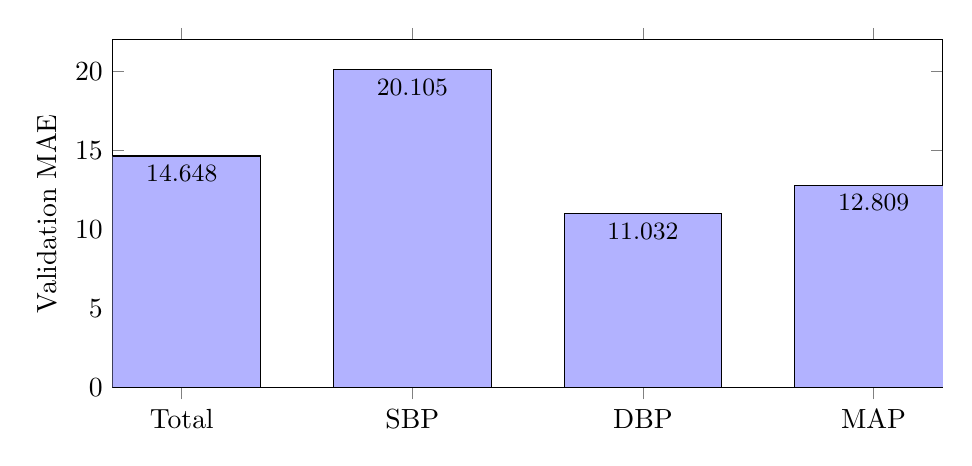
\begin{tikzpicture}
        \begin{axis}[
            width=\textwidth,
            height=6cm,
            ybar,
            ymin=0,
            ymax=22,
            bar width=2cm,
            xtick=data,
            xticklabels={Total, SBP, DBP, MAP},
            ylabel={Validation MAE},
            nodes near coords,
            nodes near coords style={font=\small, anchor=north, /pgf/number format/.cd, fixed, precision=3},
        ]
            \addplot[fill=blue!30] coordinates {(1,14.648) (2,20.105) (3,11.032) (4,12.809)};
        \end{axis}
    \end{tikzpicture}
    \captionsetup{format=plain, justification=centering, font=small}
    \caption{Average validation MAE of total, systolic, diastolic and mean arterial pressures}
    \label{fig:all_mae}
\end{figure}

The bar chart depicted in Figure~\ref{fig:all_mae} showcases the average validation MAE for distinct BP measurements.
Among the categories of Total, Systolic, Diastolic, and Mean Arterial Pressure, notable disparities in error levels were evident.

The overall average validation MAE, calculated across all models, was 14.648.
However, the individual measures displayed significant deviations.

Particularly, the most considerable MAE was observed for SBP at 20.105, indicating a pronounced level of error.
A substantial reduction in MAE was notable for DBP, nearly halving the error observed for SBP, with a recorded MAE of 11.032, marking the lowest among the measurements.
Meanwhile, MAP exhibited the second lowest MAE, closely trailing DBP at 12.809.

These findings offer valuable insights into the predictive performance of the model across distinct BP parameters,
with SBP presenting the highest margin of error, while DBP and MAP indicating relatively lower levels of error.

\begin{figure}[p]
    \centering
    \begin{minipage}{\textwidth}
        \centering
        \includegraphics[width=0.7\textwidth]{images/results/training_loss_mse}
        \vspace{0.001cm}
        \includegraphics[width=0.7\textwidth]{images/results/testing_loss_mse}
        \captionsetup{format=plain, justification=centering, font=small}
        \caption{Training and Testing Losses of LSTM \& GRU Models}
        \label{fig:train_test_mse}
    \end{minipage}
\end{figure}

\newpage


    \section{Discussion}
    \label{sec:discussion}

    Caveats:
    \begin{itemize}
        \item Out of the 34 features, 3 (delta\_t, delta\_area and res\_index) depend on the accurate detection of the dicrotic notch.
        \item Significantly more values could be extracted if finding the dicrotic notch would not be necessary.
    \end{itemize}

    % more effi sp for mimic3
    All this means is that the signal processing algorithms worked better and extracted more values from the MIMIC-III DB.
    It is also possible a hint at the fact, that the quality of the signal was better in MIMIC-III.
    This is also logical however, since there was no limit on the fetching of records from a single study or subject from MIMIC-IV,
    so huge number of segments might have been discarded, if they didn't showcase a comprehensible signal.

    % feature reduction
    It was found, that every feature contributes positively, therefore feature reduction was not applied.

    Limitations:
    \begin{itemize}
        \item Not knowing what devices were used.
        \item How they were calibrated.
        \item How accurate they are.
        \item Pulse oximeter and arterial catheter parameters.
        \item Sampling rates are different for every device (even between MIMIC 3 and 4).
    \end{itemize}

    Possible Improvements:
    \begin{itemize}
        \item Integrate both the ECG and PPG graphs for a more precise prediction.
        \item Use further signal processing approaches.
        \item Manually filter waveform graphics (e.g., faulty PPG signal).
        \item Expand on machine learning algorithms.
        \item Experiment with different median intervals.
    \end{itemize}


    \section{Conclusion}
    \label{sec:conclusion}

    Summary of findings:

    As per the joint 2018 statement by the American National Standards of the Association for the Advancement of Medical Instrumentation (AAMI), European Society of Hypertension (ESH)
    and International Organization for Standardization (ISO), the average variation and its standard deviation in NIBP measurements should ideally fall within 5 ± 8 mmHg compared to a reference BP,
    based on a minimum of 85 patient evaluations~\cite{stergiouUniversalStandardValidation2018}.

    The number of patient evaluations done in this study greatly exceed 85.
    The average variation and standard deviation of given models was: -||-

    Pretty bad performance on a huge number of data.
    Very important though, that no overfitting was done.
    Also, real-world data was simulated through MIMIC-IV (completely different data source), which is key.

    Advanced NN models performed well but not extraordinarily great.
    RF had a promising test loss, but validation loss was even worse than of LSTMs and GRUs.

    This study focused on ICU patient data, but it can prospectively be expanded on also ambulatory patients or even real-time healthy patient monitoring.

    \newpage

    \singlespacing
    \small
    \bibliographystyle{ieeetr}  % ieeetr
    \bibliography{literature_final_with_notes}
    \normalsize

    \newpage
    \appendix


    \section{Code}\label{sec:code}
    \subsection{Filters}\label{subsec:code_filters}

\begin{lstlisting}[language=Python,label={lst:filters.py}, basicstyle=\scriptsize]

from scipy.ndimage import gaussian_filter1d
import scipy as sp
import matplotlib.pyplot as plt
import numpy as np


def pre_process_data(abp, ppg, fs):
    # Gaussian filter
    g_abp = gaussian_filter1d(abp, sigma=2)
    g_ppg = gaussian_filter1d(ppg, sigma=2)

    # Gaussian Median filter
    med_a = np.median(abp)
    std_a = np.std(abp)
    sigma_a = med_a / std_a * 0.5
    gm_abp = gaussian_filter1d(abp, sigma=sigma_a)
    med_p = np.median(ppg)
    std_p = np.std(ppg)
    sigma_p = med_p / std_p * 0.3
    gm_ppg = gaussian_filter1d(ppg, sigma=sigma_p)

    # Savitzky-Golay filter
    sg_abp = filter_savgol(abp)
    sg_ppg = filter_savgol(ppg)

    # Butterworth Lowpass filter
    bl_abp = butter_lowpass_filter(abp, 5, fs, 4)
    bl_ppg = butter_lowpass_filter(ppg, 5, fs, 4)

    # Butterworth filter
    b_abp = filter_butterworth(abp, fs)
    b_ppg = filter_butterworth(ppg, fs)

    # Chebyshev Lowpass filter
    cl_abp = chebyshev2_lowpass_filter(abp, 2, fs)
    cl_ppg = chebyshev2_lowpass_filter(ppg, 2, fs)

    # Chebyshev filter
    c_abp = filter_chebyshev(abp, fs)
    c_ppg = filter_chebyshev(ppg, fs)

    # Whiskers filter
    w_abp = whiskers_filter(abp)
    w_ppg = whiskers_filter(ppg)


def filter_savgol(x):
    x_f = sp.savgol_filter(x, 51, 4)
    return x_f


def butter_lowpass_filter(data, cutoff_frequency, fs, order):
    nyquist = 0.5 * fs
    normal_cutoff = cutoff_frequency / nyquist
    b, a = sp.butter(order, normal_cutoff, btype='low', analog=False, output='ba')

    filtered_data = sp.lfilter(b, a, data)
    return filtered_data


def chebyshev2_lowpass_filter(data, cutoff_freq, fs):
    nyquist = 0.5 * fs
    normal_cutoff = cutoff_freq / nyquist
    b, a = sp.cheby2(4, 2, normal_cutoff, btype='low', analog=False)
    y = sp.lfilter(b, a, data)
    return y


def filter_butterworth(data, fs):
    lpf_cutoff = 1.25  # Hz
    hpf_cutoff = 31  # Hz
    sos_butt = sp.butter(10,
                         [lpf_cutoff, hpf_cutoff],
                         btype='bp',
                         analog=False,
                         output='sos',
                         fs=fs)
    w, h = sp.sosfreqz(sos_butt,
                       2000,
                       fs=fs)
    sos = sos_butt, w, h
    return sp.sosfiltfilt(sos[0], data)


def filter_chebyshev(data, fs):
    lpf_cutoff = 1.2  # Hz
    hpf_cutoff = 60  # Hz
    sos_cheb = sp.cheby2(4,
                         20,
                         [lpf_cutoff, hpf_cutoff],
                         btype='bp',
                         analog=False,
                         output='sos',
                         fs=fs)
    w, h = sp.sosfreqz(sos_cheb,
                       2000,
                       fs=fs)
    sos = sos_cheb, w, h
    return sp.sosfiltfilt(sos[0], data)


def whiskers_filter(data):
    bp = plt.boxplot(data)
    plt.close()

    # get lower and upper amplitude thresholds
    whiskers = [whiskers.get_ydata() for whiskers in bp['whiskers']]
    lower_amp = whiskers[0][1]
    upper_amp = whiskers[1][1]

    # get all indexes of outliers, outside the amplitude thresholds
    ind_outliers = []
    for i in range(len(data)):
        if data[i] < lower_amp or data[i] > upper_amp:
            ind_outliers.append(i)

    if len(ind_outliers) != 0:
        # get all grouped arrays with values not within the whiskers range
        ind_consecutives = []
        current_group = [ind_outliers[0]]
        for i in range(1, len(ind_outliers)):
            if ind_outliers[i] == ind_outliers[i - 1] + 1:
                current_group.append(ind_outliers[i])
            else:
                ind_consecutives.append(current_group)
                current_group = [ind_outliers[i]]
        ind_consecutives.append(current_group)

        for array_indexes in ind_consecutives:
            array_values = data[array_indexes]
            # get top (min or max) value of each consecutive group
            if array_values[0] < lower_amp:
                top_val = min(array_values)
                top_ind = array_indexes[np.argmin(array_values)]
                coef = top_val / lower_amp
            else:
                top_val = max(array_values)
                top_ind = array_indexes[np.argmax(array_values)]
                coef = top_val / upper_amp
            # calculate and (not) assign the top value according to attenuating coefficient
            adj_top_val = top_val / coef * 1.01
            if lower_amp > top_val > adj_top_val:
                continue
            if upper_amp < top_val < adj_top_val:
                continue
            data[top_ind] = adj_top_val
            # check if first group index is also first overall index
            if array_indexes[0] == 0:
                one_minus_threshold_val = data[array_indexes[0]]
                one_minus_threshold_ind = array_indexes[0]
            else:
                one_minus_threshold_val = data[array_indexes[0] - 1]
                one_minus_threshold_ind = array_indexes[0] - 1
            # check if last group index is also last overall index
            if array_indexes[-1] == len(data) - 1:
                one_plus_threshold_val = data[array_indexes[-1]]
                one_plus_threshold_ind = array_indexes[-1]
            else:
                one_plus_threshold_val = data[array_indexes[-1] + 1]
                one_plus_threshold_ind = array_indexes[-1] + 1
            # create function for calculation of other new values
            distance_to_top = top_ind - one_minus_threshold_ind
            if distance_to_top == 0:
                distance_to_top = 1
            distance_to_bottom = one_plus_threshold_ind - top_ind
            if distance_to_bottom == 0:
                distance_to_bottom = 1
            f1 = (adj_top_val - one_minus_threshold_val) / distance_to_top
            f2 = (one_plus_threshold_val - adj_top_val) / distance_to_bottom
            # assign new values
            x1, x2 = 1, 1
            for ind in array_indexes:
                if ind < top_ind:
                    data[ind] = (f1 * x1) + one_minus_threshold_val
                    x1 += 1
                elif ind > top_ind:
                    data[ind] = (f2 * x2) + adj_top_val
                    x2 += 1

    return data

\end{lstlisting}

\subsection{Beats}
\label{subsec:code_beats}

\begin{lstlisting}[language=Python,label={lst:beats.py}, basicstyle=\scriptsize]
import scipy as sp
import numpy as np


def get_optimal_beats_lists(abp, ppg, fs):
    """
    Signal processing script for examining which default beat detection algorithm is the most efficient
    :param abp: List of ABP data
    :param ppg: List of PPG data
    :param fs: Sampling frequency
    :return: Lists of optimally detected ABP and PPG pulses
    """
    abp_beats1 = pulse_detection(abp, 'd2max', len(abp) / fs, 'abp')
    ppg_beats1 = pulse_detection(ppg, 'd2max', len(ppg) / fs, 'ppg')
    abp_beats2 = pulse_detection(abp, 'upslopes', len(abp) / fs, 'abp')
    ppg_beats2 = pulse_detection(ppg, 'upslopes', len(ppg) / fs, 'ppg')
    abp_beats3 = pulse_detection(abp, 'delineator', len(abp) / fs, 'abp')
    ppg_beats3 = pulse_detection(ppg, 'delineator', len(ppg) / fs, 'ppg')

    avg1 = (len(abp_beats1) + len(ppg_beats1)) / 2
    avg2 = (len(abp_beats2) + len(ppg_beats2)) / 2
    avg3 = (len(abp_beats3) + len(ppg_beats3)) / 2

    sorted_avg = sorted([avg1, avg2, avg3])
    diff_avg12 = sorted_avg[1] - sorted_avg[0]
    diff_avg23 = sorted_avg[2] - sorted_avg[1]

    outlier = None
    if diff_avg23 > diff_avg12 * 2:
        outlier = sorted_avg[2]
    elif diff_avg12 > diff_avg23 * 2:
        outlier = sorted_avg[0]

    diff1 = abs(len(abp_beats1) - len(ppg_beats1))
    diff2 = abs(len(abp_beats2) - len(ppg_beats2))
    diff3 = abs(len(abp_beats3) - len(ppg_beats3))

    diffper1 = diff1 / avg1 * 100
    diffper2 = diff2 / avg2 * 100
    diffper3 = diff3 / avg3 * 100

    if outlier is None:
        abp_opt, ppg_opt = get_best_beats_from_diffper(diffper1, diffper2, diffper3,
                                                       abp_beats1, abp_beats2, abp_beats3,
                                                       ppg_beats1, ppg_beats2, ppg_beats3)
    else:
        if outlier == avg1:
            diffper1 = 100
        elif outlier == avg2:
            diffper2 = 100
        elif outlier == avg3:
            diffper3 = 100
        abp_opt, ppg_opt = get_best_beats_from_diffper(diffper1, diffper2, diffper3,
                                                   abp_beats1, abp_beats2, abp_beats3,
                                                   ppg_beats1, ppg_beats2, ppg_beats3)
    return abp_opt, ppg_opt


def pulse_detection(data, algorithm, duration):
    temp_fs = 125
    beats = pulse_detect(data, temp_fs, 5, algorithm, duration)
    return beats


def get_best_beats_from_diffper(diffper1, diffper2, diffper3,
                                abp_beats1, abp_beats2, abp_beats3,
                                ppg_beats1, ppg_beats2, ppg_beats3):
    smallest_diffper = min(diffper1, diffper2, diffper3)

    abp_opt = []
    ppg_opt = []

    if smallest_diffper == diffper1:
        abp_opt = abp_beats1
        ppg_opt = ppg_beats1
    elif smallest_diffper == diffper2:
        abp_opt = abp_beats2
        ppg_opt = ppg_beats2
    elif smallest_diffper == diffper3:
        abp_opt = abp_beats3
        ppg_opt = ppg_beats3

    return abp_opt, ppg_opt

def pulse_detect(x, fs, w, alg, dur):
    """
    Description: Pulse detection and correction from pulsatile signals
    Developed by: Elisa Mejia-Mejia
                   City, University of London
    Full code available at:
    https://wfdb.io/mimic_wfdb_tutorials/tutorial/notebooks/beat-detection.html
    """


def get_beats_from_mean_crossings(abp, ppg):
    mean_value = np.mean(abp)
    above_mean = abp > mean_value
    count_a = np.count_nonzero(np.diff(above_mean.astype(int)) == -1)
    mean_value = np.mean(ppg)
    above_mean = ppg > mean_value
    count_p = np.count_nonzero(np.diff(above_mean.astype(int)) == -1)
    abp_beat_interval = len(abp) / ((count_a + count_p) / 2)
    ppg_beat_interval = abp_beat_interval

    abp_beats, _ = sp.find_peaks(abp, distance=abp_beat_interval, prominence=5)
    ppg_beats, _ = sp.find_peaks(ppg, distance=ppg_beat_interval, prominence=0.01)

    return abp_beats, ppg_beats

\end{lstlisting}

\subsection{Signal Processing}
\label{subsec:code_sp}

\begin{lstlisting}[language=Python,label={lst:sp.py}, basicstyle=\scriptsize]
import numpy as np
import scipy as sp


def signal_processing(seg_name, abp, ppg, fs):
    # First iteration of beat finding (MIMIC default methods)
    abp_beats, ppg_beats = get_optimal_beats_lists(abp, ppg, seg_name)

    # For comparison: beat detection from mean crossing
    beats_a, beats_p = get_beats_from_mean_crossings(abp, ppg)
    is_larger = len(beats_a) + len(beats_p) > len(abp_beats) + len(beats_p)
    is_closer = abs(len(beats_a) - len(beats_p)) < abs(len(abp_beats) - len(ppg_beats))
    if is_larger and is_closer:
        abp_beats = beats_a
        ppg_beats = beats_p

    # Second iteration: Peak finding (SP manual methods)
    abp_beat_interval = len(abp) / len(abp_beats)
    ppg_beat_interval = len(ppg) / len(ppg_beats)
    abp_beats, _ = sp.find_peaks(abp, distance=abp_beat_interval * .75, prominence=0.5)
    ppg_beats, _ = sp.find_peaks(ppg, distance=ppg_beat_interval * .75, prominence=0.01)
    if len(abp_beats) < 100 or len(ppg_beats) < 100:
        raise Exception('Signal Processing failed: a substantial amount of beats not found')

    # Signal synchronization : delay approx = 18 (288 ms)
    abp, ppg = synchronization(abp, ppg, abp_beats, ppg_beats)

    # Third iteration: Peak finding
    abp_beats, _ = sp.find_peaks(abp, distance=abp_beat_interval * .75, prominence=0.5)
    ppg_beats, _ = sp.find_peaks(ppg, distance=ppg_beat_interval * .75, prominence=0.01)
    normal_length_a, normal_length_p = len(abp_beats), len(ppg_beats)

    # Beat grouping
    abp_beats, ppg_beats = group_beats(abp_beats, ppg_beats)

    if max(normal_length_a, normal_length_p) > max(len(abp_beats), len(ppg_beats)) * 1.05:
        raise Exception(f"too big of a difference after grouping -"
                        f"{max(normal_length_a, normal_length_p) - max(len(abp_beats), len(ppg_beats))}")

    abp_hr = round(len(abp_beats) / (len(abp) / fs) * 60, 1)
    ppg_hr = round(len(ppg_beats) / (len(ppg) / fs) * 60, 1)
    print(f"\tABP beats - {len(abp_beats)}, Heart Rate - {abp_hr}")
    print(f"\tPPG beats - {len(ppg_beats)}, Heart Rate - {ppg_hr}")

    return {
        'abp': abp,
        'ppg': ppg,
        'abp_beats': abp_beats,
        'ppg_beats': ppg_beats,
        'abp_hr': abp_hr,
        'ppg_hr': ppg_hr
    }


def synchronization(abp, ppg, abp_beats, ppg_beats):
    # Find closest PPG beat to first ABP beat
    first_ppg_ind, first_abp = None, None
    for i in range(0, len(abp_beats)):
        first_abp = abp_beats[i]
        differences = ppg_beats - first_abp
        arr = [num for num in differences if num > 0]
        if len(arr) == 0:
            raise Exception("Beat synchronisation failed: no proximal beats found")
        smallest_diff = min(arr)
        if smallest_diff < 50:
            first_ppg_ind, = np.argwhere(differences == smallest_diff)[0]
            break
    first_ppg = ppg_beats[first_ppg_ind]

    # Find closest ABP beat to last PPG beat
    last_ppg_ind = len(ppg_beats) - 1
    last_ppg = ppg_beats[last_ppg_ind]
    differences = abs(abp_beats - last_ppg)
    last_abp_ind = np.argmin(differences)
    last_abp = abp_beats[last_abp_ind]

    # Splice original ABP and PPG arrays
    new_abp = abp[first_abp:last_abp]
    new_ppg = ppg[first_ppg:last_ppg]

    return new_abp, new_ppg


def group_beats(abp_beats, ppg_beats):
    i = 0
    while i < min(len(abp_beats), len(ppg_beats)):
        a = abp_beats[i]
        p = ppg_beats[i]
        if p - 40 <= a <= p + 40:
            i += 1
        else:
            if a < p:
                abp_beats = abp_beats[abp_beats != a]
            elif a > p:
                ppg_beats = ppg_beats[ppg_beats != p]
    abp_beats, ppg_beats = equal_out_by_shortening(abp_beats, ppg_beats)
    return abp_beats, ppg_beats


def equal_out_by_shortening(a_ts, p_ts):
    if len(a_ts) > len(p_ts):
        diff = len(a_ts) - len(p_ts)
        a_ts = a_ts[:-diff]
    elif len(a_ts) < len(p_ts):
        diff = len(p_ts) - len(a_ts)
        p_ts = p_ts[:-diff]
    return a_ts, p_ts
\end{lstlisting}

\subsection{Fiducial Points}
\label{subsec:code_fidp}

\begin{lstlisting}[language=Python,label={lst:fidp.py}, basicstyle=\scriptsize]
import numpy as np
import scipy as sp


def fiducial_points(x, pks, fs, vis, header):
    """
    Description: Pulse detection and correction from pulsatile signals
    Inputs:  x, array with pulsatile signal [user defined units]
             pks, array with the position of the peaks [number of samples]
             fs, sampling rate of signal [Hz]
             vis, visualisation option [True, False]
    Outputs: fidp, dictionary with the positions of several fiducial points for the cardiac cycles [number of samples]

    Fiducial points:  1: Systolic peak (pks)
                      2: Onset, as the minimum before the systolic peak (ons)
                      3: Onset, using the tangent intersection method (ti)
                      4: Diastolic peak (dpk)
                      5: Maximum slope (m1d)
                      6: a point from second derivative PPG (a2d)
                      7: b point from second derivative PPG (b2d)
                      8: c point from second derivative PPG (c2d)
                      9: d point from second derivative PPG (d2d)
                      10: e point from second derivative PPG (e2d)
                      11: p1 from the third derivative PPG (p1)
                      12: p2 from the third derivative PPG (p2)

    Libraries: NumPy (as np), SciPy (Signal, as sp), Matplotlib (PyPlot, as plt)

    Version: 1.0 - June 2022

    Developed by: Elisa Mejía-Mejía
                   City, University of London

    Edited by: Peter Charlton (see "Added by PC")

    """
    # First, second and third derivatives
    d1x = sp.savgol_filter(x, 9, 5, deriv=1)
    d2x = sp.savgol_filter(x, 9, 5, deriv=2)
    d3x = sp.savgol_filter(x, 9, 5, deriv=3)

    # Search in time series: Onsets between consecutive peaks
    ons = np.empty(0)
    for i in range(len(pks) - 1):
        start = pks[i]
        stop = pks[i + 1]
        ibi = x[start:stop]
        aux_ons, = np.where(ibi == np.min(ibi))
        if len(aux_ons) > 1:
            aux_ons = aux_ons[0]
        ind_ons = aux_ons.astype(int)
        ons = np.append(ons, ind_ons + start)
    ons = ons.astype(int)

    # Search in time series: Diastolic peak and dicrotic notch between consecutive onsets
    dia = np.empty(0)
    dic = np.empty(0)
    for i in range(len(ons) - 1):
        start = ons[i]
        stop = ons[i + 1]
        ind_pks, = np.intersect1d(np.where(pks < stop), np.where(pks > start))
        ind_pks = pks[ind_pks]
        ibi_portion = x[ind_pks:stop]
        ibi_2d_portion = d2x[ind_pks:stop]
        aux_dic, _ = sp.find_peaks(ibi_2d_portion)
        aux_dic = aux_dic.astype(int)
        aux_dia, _ = sp.find_peaks(-ibi_2d_portion)
        aux_dia = aux_dia.astype(int)
        if len(aux_dic) != 0:
            ind_max, = np.where(ibi_2d_portion[aux_dic] == np.max(ibi_2d_portion[aux_dic]))
            aux_dic_max = aux_dic[ind_max][0]  # Adjusted by HJ
            if len(aux_dia) != 0:
                nearest = aux_dia - aux_dic_max
                aux_dic = aux_dic_max
                dic = np.append(dic, (aux_dic + ind_pks).astype(int))
                ind_dia, = np.where(nearest > 0)
                aux_dia = aux_dia[ind_dia]
                nearest = nearest[ind_dia]
                if len(nearest) != 0:
                    ind_nearest, = np.where(nearest == np.min(nearest))
                    aux_dia = aux_dia[ind_nearest]
                    dia = np.append(dia, (aux_dia + ind_pks).astype(int))
            else:
                dic = np.append(dic, (aux_dic_max + ind_pks).astype(int))
    dia = dia.astype(int)
    dic = dic.astype(int)

    # Search in D1: Maximum slope point
    m1d = np.empty(0)
    for i in range(len(ons) - 1):
        start = ons[i]
        stop = ons[i + 1]
        ind_pks, = np.intersect1d(np.where(pks < stop), np.where(pks > start))
        ind_pks = pks[ind_pks]
        ibi_portion = x[start:ind_pks]
        ibi_1d_portion = d1x[start:ind_pks]
        aux_m1d, _ = sp.find_peaks(ibi_1d_portion)
        aux_m1d = aux_m1d.astype(int)
        if len(aux_m1d) != 0:
            ind_max, = np.where(ibi_1d_portion[aux_m1d] == np.max(ibi_1d_portion[aux_m1d]))
            aux_m1d_max = aux_m1d[ind_max]
            if len(aux_m1d_max) > 1:
                aux_m1d_max = aux_m1d_max[0]
            m1d = np.append(m1d, (aux_m1d_max + start).astype(int))
    m1d = m1d.astype(int)

    # Search in time series: Tangent intersection points
    tip = np.empty(0)
    for i in range(len(ons) - 1):
        start = ons[i]
        stop = ons[i + 1]
        ibi_portion = x[start:stop]
        ibi_1d_portion = d1x[start:stop]
        low_stop = np.where(m1d < stop)  # Adjusted by HJ   ↓
        high_start = np.where(m1d > start)
        if np.intersect1d(low_stop, high_start).size == 0:
            continue
        ind_m1d, = np.intersect1d(low_stop, high_start)  #  ↑
        ind_m1d = m1d[ind_m1d] - start
        aux_tip = np.round(((ibi_portion[0] - ibi_portion[ind_m1d]) / ibi_1d_portion[ind_m1d]) + ind_m1d)
        aux_tip = aux_tip.astype(int)
        tip = np.append(tip, (aux_tip + start).astype(int))
    tip = tip.astype(int)

    # Search in D2: A, B, C, D and E points
    a2d = np.empty(0)
    b2d = np.empty(0)
    c2d = np.empty(0)
    d2d = np.empty(0)
    e2d = np.empty(0)
    for i in range(len(ons) - 1):
        start = ons[i]
        stop = ons[i + 1]
        ibi_portion = x[start:stop]
        ibi_1d_portion = d1x[start:stop]
        ibi_2d_portion = d2x[start:stop]
        ind_m1d = np.intersect1d(np.where(m1d > start), np.where(m1d < stop))
        ind_m1d = m1d[ind_m1d]
        aux_m2d_pks, _ = sp.find_peaks(ibi_2d_portion)
        aux_m2d_ons, _ = sp.find_peaks(-ibi_2d_portion)
        if len(aux_m2d_pks) == 0 or len(aux_m2d_ons) == 0:  # Augmented by HJ
            continue
        # a point:
        ind_a, = np.where(ibi_2d_portion[aux_m2d_pks] == np.max(ibi_2d_portion[aux_m2d_pks]))
        ind_a = aux_m2d_pks[ind_a]
        ind_a = ind_a[0]  # Adjusted by HJ
        if (ind_a < ind_m1d):
            a2d = np.append(a2d, ind_a + start)
            # b point:
            ind_b = np.where(ibi_2d_portion[aux_m2d_ons] == np.min(ibi_2d_portion[aux_m2d_ons]))
            ind_b = aux_m2d_ons[ind_b]
            ind_b = ind_b[0]  # Adjusted by HJ
            if (ind_b > ind_a) and (ind_b < len(ibi_2d_portion)):
                b2d = np.append(b2d, ind_b + start)
        # e point:
        if len(ind_m1d) == 0: # Augmented by HJ
            continue
        ind_e, = np.where(aux_m2d_pks > ind_m1d - start)
        aux_m2d_pks = aux_m2d_pks[ind_e]
        ind_e, = np.where(aux_m2d_pks < 0.6 * len(ibi_2d_portion))
        ind_e = aux_m2d_pks[ind_e]
        if len(ind_e) >= 1:
            if len(ind_e) >= 2:
                ind_e = ind_e[1]
            e2d = np.append(e2d, ind_e + start)
            # c point:
            ind_c, = np.where(aux_m2d_pks < ind_e)
            if len(ind_c) != 0:
                ind_c_aux = aux_m2d_pks[ind_c]
                ind_c, = np.where(ibi_2d_portion[ind_c_aux] == np.max(ibi_2d_portion[ind_c_aux]))
                ind_c = ind_c_aux[ind_c]
                if len(ind_c) != 0:
                    c2d = np.append(c2d, ind_c + start)
            else:
                aux_m1d_ons, _ = sp.find_peaks(-ibi_1d_portion)
                ind_c, = np.where(aux_m1d_ons < ind_e)
                ind_c_aux = aux_m1d_ons[ind_c]
                if len(ind_c) != 0:
                    ind_c, = np.where(ind_c_aux > ind_b)
                    ind_c = ind_c_aux[ind_c]
                    if len(ind_c) > 1:
                        ind_c = [ind_c[0]]  # Adjusted by HJ
                    c2d = np.append(c2d, ind_c + start)
            # d point:
            if len(ind_c) != 0:
                ind_d = np.intersect1d(np.where(aux_m2d_ons < ind_e), np.where(aux_m2d_ons > ind_c))
                if len(ind_d) != 0:
                    ind_d_aux = aux_m2d_ons[ind_d]
                    ind_d, = np.where(ibi_2d_portion[ind_d_aux] == np.min(ibi_2d_portion[ind_d_aux]))
                    ind_d = ind_d_aux[ind_d]
                    if len(ind_d) != 0:
                        d2d = np.append(d2d, ind_d + start)
                else:
                    ind_d = ind_c
                    d2d = np.append(d2d, ind_d + start)
    a2d = a2d.astype(int)
    b2d = b2d.astype(int)
    c2d = c2d.astype(int)
    d2d = d2d.astype(int)
    e2d = e2d.astype(int)

    # Search in D3: P1 and P2 points
    p1p = np.empty(0)
    p2p = np.empty(0)
    for i in range(len(ons) - 1):
        start = ons[i]
        stop = ons[i + 1]
        ibi_portion = x[start:stop]
        ibi_1d_portion = d1x[start:stop]
        ibi_2d_portion = d2x[start:stop]
        ibi_3d_portion = d3x[start:stop]
        ind_b = np.intersect1d(np.where(b2d > start), np.where(b2d < stop))
        ind_b = b2d[ind_b]
        ind_c = np.intersect1d(np.where(c2d > start), np.where(c2d < stop))
        ind_c = c2d[ind_c]
        ind_d = np.intersect1d(np.where(d2d > start), np.where(d2d < stop))
        ind_d = d2d[ind_d]
        ind_dic = np.intersect1d(np.where(dic > start), np.where(dic < stop))
        ind_dic = dic[ind_dic]
        aux_p3d_pks, _ = sp.find_peaks(ibi_3d_portion)
        aux_p3d_ons, _ = sp.find_peaks(-ibi_3d_portion)
        # P1:
        if (len(aux_p3d_pks) != 0 and len(ind_b) != 0):
            ind_p1, = np.where(aux_p3d_pks > ind_b - start)
            if len(ind_p1) != 0:
                ind_p1 = aux_p3d_pks[ind_p1[0]]
                p1p = np.append(p1p, ind_p1 + start)
        # P2:
        if (len(aux_p3d_ons) != 0 and len(ind_c) != 0 and len(ind_d) != 0):
            if ind_c == ind_d:
                ind_p2, = np.where(aux_p3d_ons > ind_d - start)
                if len(ind_p2) == 0:  # Augmented by HJ
                    continue
                ind_p2 = aux_p3d_ons[ind_p2[0]]
            else:
                ind_p2, = np.where(aux_p3d_ons < ind_d - start)
                if len(ind_p2) == 0: # Augmented by HJ
                    continue
                ind_p2 = aux_p3d_ons[ind_p2[-1]]
            if len(ind_dic) != 0:
                aux_x_pks, _ = sp.find_peaks(ibi_portion)
                if ind_p2 > ind_dic - start:
                    ind_between = np.intersect1d(np.where(aux_x_pks < ind_p2), np.where(aux_x_pks > ind_dic - start))
                else:
                    ind_between = np.intersect1d(np.where(aux_x_pks > ind_p2), np.where(aux_x_pks < ind_dic - start))
                if len(ind_between) != 0:
                    ind_p2 = aux_x_pks[ind_between[0]]
            p2p = np.append(p2p, ind_p2 + start)
    p1p = p1p.astype(int)
    p2p = p2p.astype(int)

    off = ons[1:]
    ons = ons[:-1]
    if pks[0] < ons[0]:
        pks = pks[1:]
    if pks[-1] > off[-1]:
        pks = pks[:-1]

    # Creation of dictionary
    fidp = {'pks': pks.astype(int),
            'ons': ons.astype(int),
            'off': off.astype(int),
            'tip': tip.astype(int),
            'dia': dia.astype(int),
            'dic': dic.astype(int),
            'm1d': m1d.astype(int),
            'a2d': a2d.astype(int),
            'b2d': b2d.astype(int),
            'c2d': c2d.astype(int),
            'd2d': d2d.astype(int),
            'e2d': e2d.astype(int),
            'p1p': p1p.astype(int),
            'p2p': p2p.astype(int)
            }

    return fidp

\end{lstlisting}

\subsection{Feature Extraction}
\label{subsec:code_fe}

\begin{lstlisting}[language=Python,label={lst:fe.py}, basicstyle=\scriptsize]
import numpy as np
from scipy.integrate import simps


def sys_dia_detection(fidp, data):
    # (From filtered data) Systolic BP = pks; Diastolic BP = dia
    sys = fidp['pks']
    dia = fidp['off']
    sys, dia = group_sys_dia(sys, dia)
    length = min(len(sys), len(dia))
    tss = np.zeros(length, dtype=int)
    tsd = np.zeros(length, dtype=int)
    sysv = np.zeros(length, dtype=float)
    diav = np.zeros(length, dtype=float)
    beat_no, adj_beat_no = 0, 0
    while beat_no < len(tss):
        sys_beat = data[sys[beat_no + adj_beat_no]]
        dia_beat = data[dia[beat_no + adj_beat_no]]
        if sys_beat >= dia_beat:
            tss[beat_no] = sys[beat_no + adj_beat_no]
            sysv[beat_no] = sys_beat
            tsd[beat_no] = dia[beat_no + adj_beat_no]
            diav[beat_no] = dia_beat
            beat_no += 1
        else:
            tss = np.delete(tss, beat_no)
            sysv = np.delete(sysv, beat_no)
            tsd = np.delete(tsd, beat_no)
            diav = np.delete(diav, beat_no)
            adj_beat_no += 1
    sys = np.column_stack((tss, sysv))
    dia = np.column_stack((tsd, diav))
    return sys, dia, tss, sysv, tsd, diav


def systolic_time_detection(f_pks, f_ons, pk_index, data, fs):
    # Systolic Time = Systolic peak - Onset
    value = (f_pks[pk_index] - f_ons[pk_index]) / fs
    # Systolic Area = Integral of PPG with limits [ons:pks]
    time_interval_start, time_interval_end = f_ons[pk_index], f_pks[pk_index]
    time_interval = np.arange(time_interval_start, time_interval_end)
    signal_interval = data[time_interval_start:time_interval_end]
    area = simps(signal_interval, time_interval)
    return value, area


def diastolic_time_detection(f_off, f_pks, pk_index, data, fs):
    # Diastolic Time = Offset - Systolic peak
    value = (f_off[pk_index] - f_pks[pk_index]) / fs
    # Diastolic Area = Integral of PPG with limits [pks:off]
    time_interval_start, time_interval_end = f_pks[pk_index], f_off[pk_index]
    time_interval = np.arange(time_interval_start, time_interval_end)
    signal_interval = data[time_interval_start:time_interval_end]
    area = simps(signal_interval, time_interval)
    return value, area


def delta_t_detection(f_dia, f_pks, pk_index, data, fs):
    # delta T = Dicrotic notch - Systolic peak
    value = (f_dia[pk_index] - f_pks[pk_index]) / fs
    # Delta Area = Integral of PPG with limits [pks:dia]
    time_interval_start, time_interval_end = f_pks[pk_index], f_dia[pk_index]
    time_interval = np.arange(time_interval_start, time_interval_end)
    signal_interval = data[time_interval_start:time_interval_end]
    abs_time_interval = np.arange(0, len(signal_interval))
    area = simps(signal_interval, abs_time_interval)
    return value, area


def pulse_area_detection(f_ons, f_off, pk_index, data):
    # Pulse Area = Integral of PPG with limits [ons:off]
    time_interval_start, time_interval_end = f_ons[pk_index], f_off[pk_index]
    time_interval = np.arange(time_interval_start, time_interval_end)
    signal_interval = data[time_interval_start:time_interval_end]
    value = simps(signal_interval, time_interval)
    return value


def resistive_index_detection(f_dia, f_pks, f_off, pk_index, data):
    # RI = (data[dia] - data[off]) / (data[pks] - data[off])
    h1 = data[f_dia[pk_index]] - data[f_off[pk_index]]
    h2 = data[f_pks[pk_index]] - data[f_off[pk_index]]
    value = h1 / h2
    return value


def vessel_volume_index_detection(f_pks, f_off, pk_index, data):
    # Vessel Volume Fill-Up (systolic) Index = data[pks] / max(data[all_systoles])
    max_v = max(data[f_pks[f_pks != 0]])
    v1 = data[f_pks[pk_index]] / max_v
    # Vessel Volume Drained (diastolic) Index = max(data[all_systoles]) / data[off]
    min_v = min(data[f_off[f_off != 0]])
    v2 = min_v / data[f_off[pk_index]]
    return v1, v2


def systolic_diastolic_width_detection(f_ons, f_pks, f_off, pk_index, data, fs, p):
    # Systolic width = data[(data[pks]-data[ons])*p/100]
    ind_ons, ind_pk, ind_off = f_ons[pk_index], f_pks[pk_index], f_off[pk_index]
    val_ons, val_pk, val_off = data[ind_ons], data[ind_pk], data[ind_off]
    threshold = p / 100 * (val_pk - val_ons) + val_ons
    sys_arr = np.abs(np.array(data[ind_ons:ind_pk]) - threshold)
    ind_sw = np.argmin(sys_arr)
    sw = (len(sys_arr) - 1 - ind_sw) / fs
    dia_arr = np.abs(np.array(data[ind_pk:ind_off]) - threshold)
    ind_dw = np.argmin(dia_arr)
    dw = (ind_dw - 0) / fs
    return sw, dw


def frequency_domain_features(signal, fs):
    # Compute the Fast Fourier Transform (FFT)
    fft_result = np.fft.fft(signal)
    # Compute the frequencies corresponding to the FFT result
    frequencies = np.fft.fftfreq(len(fft_result), 1 / fs)
    # Only consider positive frequencies
    positive_frequencies = frequencies[:len(frequencies) // 2]
    # Magnitude spectrum (absolute values of FFT result)
    magnitude_spectrum = np.abs(fft_result[:len(fft_result) // 2])
    # Find the index corresponding to the maximum magnitude
    peak_frequency_index = np.argmax(magnitude_spectrum)
    # Other frequency domain features
    mean_frequency = np.sum(positive_frequencies * magnitude_spectrum) / np.sum(magnitude_spectrum)
    total_power = np.sum(magnitude_spectrum)
    normalized_power_at_peak = magnitude_spectrum[peak_frequency_index] / total_power
    return {
        'mean_frequency': mean_frequency,
        'total_power': total_power,
        'normalized_power_at_peak': normalized_power_at_peak
    }
\end{lstlisting}

\subsection{Machine Learning}
\label{subsec:code_ml}

\begin{lstlisting}[language=Python,label={lst:ml.py}, basicstyle=\scriptsize]
import torch
import torch.nn as nn
import sklearn


class LinearRegression(nn.Module):
    def __init__(self, input_size, output_size):
        super(LinearRegression, self).__init__()
        self.linear = nn.Linear(input_size, output_size)

    def forward(self, x):
        return self.linear(x)


class NeuralNet(nn.Module):
    def __init__(self, input_size, hidden_size, output_size):
        super(NeuralNet, self).__init__()
        self.input_size = input_size
        self.l1 = nn.Linear(input_size, hidden_size)
        self.relu = nn.ReLU()
        self.l2 = nn.Linear(hidden_size, output_size)

    def forward(self, x):
        out = self.l1(x)
        out = self.relu(out)
        out = self.l2(out)
        return out


class LSTM(nn.Module):
    def __init__(self, input_size, hidden_size, out_features, feature_importances):
        super(LSTM, self).__init__()
        self.hidden_size = hidden_size
        self.lstm1 = nn.LSTMCell(input_size, hidden_size)
        self.lstm2 = nn.LSTMCell(hidden_size, hidden_size)
        self.linear = nn.Linear(hidden_size, out_features)
        self.feature_importances = feature_importances

    def forward(self, x):
        h_t = torch.zeros(x.size(0), self.hidden_size, dtype=torch.float32)
        c_t = torch.zeros(x.size(0), self.hidden_size, dtype=torch.float32)
        h_t2 = torch.zeros(x.size(0), self.hidden_size, dtype=torch.float32)
        c_t2 = torch.zeros(x.size(0), self.hidden_size, dtype=torch.float32)
        adjusted_input = x * self.feature_importances.unsqueeze(0)
        h_t, c_t = self.lstm1(adjusted_input, (h_t, c_t))
        h_t2, c_t2 = self.lstm2(h_t, (h_t2, c_t2))
        output = self.linear(h_t2)
        return output


class GRU(nn.Module):
    def __init__(self, input_size, hidden_size, out_features):
        super(GRU, self).__init__()
        self.hidden_size = hidden_size
        self.gru1 = nn.GRUCell(input_size, hidden_size)
        self.gru2 = nn.GRUCell(hidden_size, hidden_size)
        self.linear = nn.Linear(hidden_size, out_features)

    def forward(self, x):
        h_t = torch.zeros(x.size(0), self.hidden_size, dtype=torch.float32)
        h_t2 = torch.zeros(x.size(0), self.hidden_size, dtype=torch.float32)
        h_t = self.gru1(x, h_t)
        h_t2 = self.gru2(h_t, h_t2)
        output = self.linear(h_t2)
        return output

# Support Vector Regression
svr_model = sklearn.svm.SVR(kernel='linear', C=100, epsilon=0.1)

# Random Forest Regressor
rf_model = sklearn.ensemble.RandomForestRegressor(n_estimators=100, max_depth=10, min_samples_split=2)
\end{lstlisting}

    \newpage

    \section{ML Results}\label{sec:ml_results}
    \subsection{ML Model Performance Measures}\label{subsec:misc_measures}

\onehalfspacing

\begin{verbatim}
INFO - PyTorch LR: learning_rate=0.01,
    epochs=10000 (SYS, DIA, MAP from 34 Median PPG Features)
    MSE: 217.2289, RMSE: 14.7387, MAE: 11.091,
    R^2: 0.062, Bias: -0.012, LoA: (-28.902, 28.877)
\end{verbatim}

\begin{verbatim}
INFO - PyTorch LR (WA): learning_rate=0.01,
    epochs=10000 (SYS, DIA, MAP from 34 Median PPG Features)
    MSE: 217.2582, RMSE: 14.7397, MAE: 11.093,
    R^2: 0.063, Bias: -0.019, LoA: (-28.910, 28.873)
\end{verbatim}

\begin{verbatim}
INFO - PyTorch MLP: learning_rate=0.01,
    epochs=10000 (SYS, DIA, MAP from 34 Median PPG Features)
    MSE: 196.1354, RMSE: 14.0048, MAE: 10.567,
    R^2: 0.152, Bias: 0.046, LoA: (-27.405, 27.497)
\end{verbatim}

\begin{verbatim}
INFO - PyTorch MLP (WA): learning_rate=0.01,
    epochs=10000 (SYS, DIA, MAP from 34 Median PPG Features)
    MSE: 249.7456, RMSE: 15.8033, MAE: 11.802,
    R^2: -0.072, Bias: -1.373, LoA: (-32.233, 29.486)
\end{verbatim}

\begin{verbatim}
INFO - PyTorch LSTM: learning_rate=0.1,
    epochs=100 (SYS, DIA, MAP from 34 Median PPG Features)
    MSE: 101.4742, RMSE: 10.0734, MAE: 7.119,
    R^2: 0.556, Bias: -0.034, LoA: (-19.779, 19.711)
\end{verbatim}

\begin{verbatim}
INFO - PyTorch LSTM (WA): learning_rate=0.1,
    epochs=100 (SYS, DIA, MAP from 34 Median PPG Features)
    MSE: 143.2955, RMSE: 11.9706, MAE: 8.697,
    R^2: 0.373, Bias: 0.056, LoA: (-23.408, 23.520)
\end{verbatim}

\begin{verbatim}
INFO - PyTorch Bi-LSTM: learning_rate=0.1,
    epochs=100 (SYS, DIA, MAP from 34 Median PPG Features)
    MSE: 118.1035, RMSE: 10.8675, MAE: 7.850,
    R^2: 0.481, Bias: 0.114, LoA: (-21.187, 21.414)
\end{verbatim}

\begin{verbatim}
INFO - PyTorch Bi-LSTM (WA): learning_rate=0.1,
    epochs=100 (SYS, DIA, MAP from 34 Median PPG Features)
    MSE: 159.7223, RMSE: 12.6381, MAE: 9.362,
    R^2: 0.303, Bias: -0.005, LoA: (-24.778, 24.767)
\end{verbatim}

\begin{verbatim}
INFO - PyTorch GRU: learning_rate=0.1,
    epochs=100 (SYS, DIA, MAP from 34 Median PPG Features)
    MSE: 93.5903, RMSE: 9.6742, MAE: 6.823,
    R^2: 0.587, Bias: -0.034, LoA: (-18.997, 18.928)
\end{verbatim}

\begin{verbatim}
INFO - PyTorch GRU (WA): learning_rate=0.1,
    epochs=100 (SYS, DIA, MAP from 34 Median PPG Features)
    MSE: 142.1063, RMSE: 11.9208, MAE: 8.658,
    R^2: 0.377, Bias: -0.059, LoA: (-23.425, 23.308)
\end{verbatim}

\begin{verbatim}
INFO - PyTorch Bi-GRU: learning_rate=0.1,
    epochs=100 (SYS, DIA, MAP from 34 Median PPG Features)
    MSE: 117.7146, RMSE: 10.8496, MAE: 7.844,
    R^2: 0.482, Bias: 0.034, LoA: (-21.233, 21.300)
\end{verbatim}

\begin{verbatim}
INFO - PyTorch Bi-GRU (WA): learning_rate=0.1,
    epochs=100 (SYS, DIA, MAP from 34 Median PPG Features)
    MSE: 173.8695, RMSE: 13.1860, MAE: 9.811,
    R^2: 0.241, Bias: -0.087, LoA: (-25.933, 25.759)
\end{verbatim}

\begin{verbatim}
INFO - RF (SYS, DIA, MAP from 34 Median PPG Features)
    MSE: 66.383, MAE: 5.075,
    R^2: 0.713, Bias: 0.069,
    LoA: [16.037, 16.037]
\end{verbatim}

\newpage

\subsection{Feature Importance Plots}\label{subsec:plots_fi}

\begin{figure}[b!]
    \centering
    \hspace{-2cm}
    \includegraphics[width=0.82\textwidth]{images/results/feature_importance/feature_importance_plot_LR_0}
    \caption{Feature Importance Chart LR}
    \label{fig:fi_lr}
\end{figure}

\begin{figure}[h]
    \centering
    \vspace{-1cm}
    \hspace{-2cm}
    \includegraphics[width=\textwidth]{images/results/feature_importance/feature_importance_plot_MLP_0}
    \caption{Feature Importance Chart MLP}
    \label{fig:fi_mlp}
\end{figure}

\begin{figure}[h]
    \centering
    \vspace{-1cm}
    \hspace{-2cm}
    \includegraphics[width=\textwidth]{images/results/feature_importance/feature_importance_plot_LSTM_0}
    \caption{Feature Importance Chart LSTM}
    \label{fig:fi_lstm}
\end{figure}

\begin{figure}[h]
    \centering
    \vspace{-1cm}
    \hspace{-2cm}
    \includegraphics[width=\textwidth]{images/results/feature_importance/feature_importance_plot_Bi-LSTM_0}
    \caption{Feature Importance Chart Bi-LSTM}
    \label{fig:fi_bi_lstm}
\end{figure}

\begin{figure}[h]
    \centering
    \vspace{-1cm}
    \hspace{-2cm}
    \includegraphics[width=\textwidth]{images/results/feature_importance/feature_importance_plot_GRU_0}
    \caption{Feature Importance Chart GRU}
    \label{fig:fi_gru}
\end{figure}

\begin{figure}[h]
    \centering
    \vspace{-1cm}
    \hspace{-2cm}
    \includegraphics[width=\textwidth]{images/results/feature_importance/feature_importance_plot_Bi-GRU_0}
    \caption{Feature Importance Chart Bi-GRU}
    \label{fig:fi_bi_gru}
\end{figure}

\end{document}